\documentclass[12pt,a4paper]{ufpr}

%\usepackage{silence}
%\WarningsOff
%\WarningsOff[latex]


\usepackage[brazil]{babel}
\usepackage[T1]{fontenc}
\usepackage[latin1]{inputenc}

\usepackage{pdflscape}
\usepackage[shortcuts]{extdash}
\usepackage[bottom]{footmisc}
\usepackage{amssymb,amsmath}
\usepackage{isolatin1}
\usepackage{amssymb}
\usepackage{subfigure}
\usepackage[hypcap]{caption}
\usepackage{setspace}
\usepackage{ps-macros}
\usepackage{tabularx}
\usepackage{tabulary}
\usepackage[table]{xcolor}
\usepackage{float}

\usepackage[nomain,nonumberlist,acronym]{glossaries}
\loadglsentries[\acronymtype]{abreviacoes}
%\makeglossaries

\usepackage[hidelinks]{hyperref}
\usepackage{booktabs}
\usepackage{multirow}
\usepackage{rotating}
\usepackage{pdflscape}

\usepackage{graphicx}
\graphicspath{{./Imagens/}}
\DeclareGraphicsExtensions{.png,.jpg}

\usepackage[onelanguage,portuguese,algochapter,linesnumbered,ruled,inoutnumbered]{algorithm2e}
\usepackage{algorithm2eportuguese}

\usepackage{xcolor,colortbl}

\usepackage{syntax}
\grammarindent 80pt

\usepackage{newfloat}
% declare the floating environment {Grammar}
% this will also define \listofGrammars:
\DeclareFloatingEnvironment[
% the file extension for the file used to create the list:
fileext   = logr,% don't use log here!
% the heading for the list:
listname  = {List of Grammars},
% the name used in captions:
name      = Gram�tica,
% the default floating parameters if the environment is used
% without optional argument:
placement = htp
]{Grammar}





\newcommand{\mc}[2]{\multicolumn{#1}{c}{#2}}
\definecolor{Gray}{gray}{0.85}
\definecolor{LightCyan}{rgb}{0.88,1,1}

\newcolumntype{a}{>{\columncolor{Gray}}c}
\newcolumntype{b}{>{\columncolor{white}}c}

\linespread{1.3}
\setcounter{secnumdepth}{3}
\setcounter{tocdepth}{3}

\title{Uma proposta de design autom�tico de heur�sticas alto n�vel para um \textit{framework} hiper-heur�stico aplicado ao problema de dobramento de prote�nas utilizando o modelo hp 2d}
\author{Vidal Daniel da Fontoura}
\advisortitle{Orientadora} % ou Orientador
\advisorname{Prof.$^a$ Dr.$^a$ Aurora Trinidad Ramirez Pozo }
\advisorplace{Departamento de Inform�tica, UFPR}  % departamento, instituicao
\city{Curitiba - PR}
\year{2015}

%\banca        % nao insira o nome do orientador, ja eh feito automaticamente
%:{Prof.$^a$ Me.$^a$ Thelma Elita Colanzi Lopes}{Departamento de Inform�tica, UEM}
%{Prof. Dr. Marcos Didonet Del Fabro}{Departamento de Inform�tica, UFPR}
{}{} % se nao houver deixe em branco {}{}
{}{}    % se houver um quarto membro na banca, inserir nome e instituicao

%\defesa{02 de agosto de 2014} % dia em que foi realizada a defesa da dissertacao

%\makeglossary

\begin{document}

\pdfstringdefDisableCommands{
	\let\MakeUppercase\relax
}

\makecapaproposta             % cria capa para proposta%
%\makecapadissertacao           % cria capa para dissertacao de mestrado %
%\makerosto                     % cria folha de rosto para versao final da UFPR %
%\maketermo                     % cria folha com o termo de aprovacao da dissertacao%

%\singlespacing           % espacamento 1 - capa UFPR%
%\onehalfspacing          % espacamento 1/2 %
\doublespacing            % espacamento 2 - UFPR %

\pagestyle{headings}
\pagenumbering{roman}

\tableofcontents

%\chapter*{Resumo}
\addcontentsline{toc}{chapter}{RESUMO}

Prote�nas s�o estruturas, compostas por amino�cidos, que exercem um papel de suma import�ncia na natureza. Estas estruturas s�o formadas a partir de um processo de dobramento, onde uma sequ�ncia de amino�cidos inicialmente desdobrada ir� adotar uma conforma��o/estrutura espacial �nica/nativa. Entretanto, o processo de dobramento ainda n�o � completamente compreendido e � considerado um dos maiores desafios das �reas de biologia, qu�mica, medicina e bioinform�tica. Este desafio � conhecido como o problema de dobramento de prote�nas (PDP) e trata da predi��o de estruturas de prote�nas. Christian Anfinsen et al. \cite{anfinsen1972studies} descrevem que o PDP pode ser visto como um problema de minimiza��o, pois afirmam que a estrutura nativa de uma prote�na � aquela que minimiza sua energia global livre. Dessa maneira, diversas estrat�gias heur�sticas utilizando modelos simplificados de representa��o de prote�nas, tais como modelo HP, vem sendo desenvolvidas para buscar a estrutura nativa de prote�nas. Por se tratar de um problema complexo com muitos m�nimos locais e restri��es, surge a demanda de estrat�gias que possuam mecanismos robustos para manter a diversidade assim como intensificar a busca quando necess�rio. � nesse contexto que hiper-heur�sticas se apresentam como boas op��es para explorar o espa�o de busca de problemas complexos. Nesta proposta, � descrita uma estrat�gia de gera��o de heur�sticas de alto n�vel utilizando uma t�cnica de programa��o gen�tica chamada evolu��o gramatical, a qual utiliza uma gram�tica BNF para gerar programas de computador. Um conjunto terminal e n�o terminal foi desenvolvido, baseado no trabalho de Sabar e colaboradores, e uma gram�tica espec�fica para decodificar vetores de inteiros em heur�sticas de alto n�vel. A evolu��o gramatical utiliza um processo evolutivo para evoluir uma popula��o de programas. As heur�sticas de alto n�vel ir�o compor uma plataforma hiper-heur�stica, a qual tamb�m possuir� um conjunto de heur�sticas de baixo n�vel e um mecanismo de mem�ria de solu��es ao PDP. A estrat�gia proposta ser� aplicada utilizando um conjunto de \text{benchmark} com diferentes sequ�ncias de amino�cidos e comparada com outros trabalhos que utilizam o mesmo conjunto de \textit{benchmark}.



\newpage

%\chapter*{Abstract}
%\addcontentsline{toc}{chapter}{\MakeUppercase{Abstract}}
%%\input{abstract.tex}        % somente o texto
%\newpage

\addcontentsline{toc}{chapter}{LISTA DE FIGURAS}
\listoffigures
\newpage

\addcontentsline{toc}{chapter}{LISTA DE TABELAS}
\listoftables
\newpage

\addcontentsline{toc}{chapter}{GLOSS�RIO}
\newglossarystyle{mylist}{%
	\glossarystyle{index}% base this style on the list style
	\renewcommand{\glsgroupskip}{}% make nothing happen
}
\printglossary[type=\acronymtype,title=GLOSS�RIO,style=mylist]
\newpage

% Cap�tulos
\pagenumbering{arabic}

%\input{aspectos}

\chapter{Introdu��o}
\label{Introducao}

Prote�nas exercem um papel fundamental na natureza, participando em muitas fun��es importantes das c�lulas vivas. Prote�nas s�o estruturas que garantem o correto funcionamento de um amplo n�mero de entidades biol�gicas. Estas estruturas s�o resultados de um processo chamado dobramento de prote�nas, no qual uma cadeia de amino�cidos inicialmente desdobrada ser� transformada em sua estrutura final/nativa. A predi��o de estruturas de prote�nas possui um campo amplo de aplica��es biotecnol�gicas e m�dicas. Por exemplo: design de novas prote�nas e dobramentos \cite{wang2012structural, rothlisberger2008kemp}, s�ntese de novas drogas baseada nas estruturas \cite{qian2004improvement, krieger2009improving}  e obten��o experimental de estruturas a partir de dados incompletos de resson�ncia magn�tica nuclear \cite{shen2009novo}.  
A determina��o da estrutura nativa de prote�nas � uma tarefa desafiadora at� mesmo para modernos super computadores. Isto ocorre por conta do imenso espa�o de busca para testar todas as poss�veis configura��es que uma dada prote�na pode adotar. Diferentes formas de representar as estruturas/conforma��es de prote�nas existem e podem ser utilizadas para simular o processo de dobramento. Embora existam modelos extremamente detalhados, estas representa��es s�o computacionalmente muito custosas. Consequentemente, muitos autores \cite{custodio2004investigation,hsu2003growth,lin2011protein,unger1993genetic,santanna2008,custodio2014multiple, garza2012locality} utilizam modelos simplificados para representar as estruturas de prote�nas. Um modelo bastante conhecido para este prop�sito, criado por Lau and Dill \cite{lau1989lattice}, � o modelo Hidrof�bico-Polar (HP). Este modelo generaliza os amino�cidos que comp�em as prote�nas em apenas dois tipos H ou P. Geralmente  utiliza-se um \textit{grid} (2D) ou cubo (3D) para representar as poss�veis conforma��es que uma dada prote�na pode obter a partir do processo de dobramento. Para avaliar as estruturas representadas pelo modelo HP � preciso computar o valor de energia associado a uma dada conforma��o. Para isto, � necess�rio considerar as intera��es entre os amino�cidos. Uma intera��o ocorre quando o par de amino�cidos � adjacente no \textit{grid}/cubo e n�o � adjacente na sequ�ncia. No modelo HP existem apenas tr�s: (HP, HH e PP), mas somente intera��es hidrof�bicas (HH) influenciam no valor de energia referente a uma conforma��o. A quest�o que surge � como buscar, dentre as poss�veis conforma��es, aquela cuja a energia seja m�nima.
Diferentes estrat�gias heur�sticas t�m sido desenvolvidas para diminuir a complexidade para encontrar conforma��es onde a energia seja m�nima utilizando modelos simplificados. Estas abordagens utilizam t�cnicas como algoritmos gen�ticos, otimiza��o de col�nia de formigas, algoritmos de estima��o de distribui��o, otimiza��o por enxame de part�culas e algoritmos evolucion�rios multiobjetivos dentre outras. 
Esta proposta visa a aplica��o de uma estrat�gia de gera��o autom�tica dos componentes de alto n�vel para um \textit{framework} hiper-heur�stico, utilizando evolu��o gramatical (EG) que trata-se de uma t�cnica de programa��o gen�tica (PG). Pretende-se utilizar a EG para gerar mecanismos de sele��o e crit�rios de aceita��o para um \textit{framework} hiper-heur�stico aplicado ao problema de dobramento de prote�nas (PDP).

 
 
\section{Organiza��o do Texto}
\label{Introducao:Organizacao do Texto}

O restante dessa proposta est� organizado da seguinte maneira: no cap�tulo \ref{Referencial Teorico} � introduzido o referencial te�rico necess�rio para uma boa compreens�o sobre hiper-heur�sticas, sua classifica��o e tamb�m os conceitos de programa��o gen�tica (PG) e evolu��o gramatical (EG). Em seguida, no cap�tulo \ref{Problema de Dobramento de Prote�nas} � apresentado o problema de dobramento de prote�nas e seus aspectos relevantes. Na sequ�ncia, o cap�tulo \ref{Trabalhos Relacionados} apresenta alguns trabalhos relacionados com esta proposta. A metodologia proposta � apresentada no cap�tulo \ref{Metodologia}. Por fim, o cronograma desta proposta � apresentado no cap�tulo \ref{Proposta de Trabalho}
\chapter{Referencial Te�rico}
\label{Referencial Teorico}

Este cap�tulo tem como objetivo apresentar o referencial te�rico necess�rio para o desenvolvimento e entendimento deste trabalho, introduzindo conceitos sobre hiper-heur�sticas, programa��o gen�tica, e evolu��o gramatical. As Se��es~\ref{Hiper-Heuristicas},~\ref{Hiper-Heuristicas-Sele��o} e~\ref{Hiper-Heuristicas-Gera�ao} apresentam o conte�do necess�rio para o entendimento sobre hiper-heur�sticas, a Se��o~\ref{subsection:PG} introduz o conceito e aspectos referentes � programa��o gen�tica, a Se��o~\ref{subsubsection:EvolucaoGramatical} apresenta a evolu��o gramatical e por fim a Se��o~\ref{subsubsection:PGasHH} descreve como utilizar programa��o gen�tica como uma hiper-heur�stica de gera��o.

\section{Hiper-Heur�sticas }
\label{Hiper-Heuristicas}

Apesar do sucesso de m�todos heur�sticos e outros m�todos de busca na tarefa de resolver dif�ceis problemas de busca computacional ainda existem dificuldades em generalizar estes m�todos para diferentes problemas ou at� mesmo para diferentes inst�ncias de um mesmo problema. Esta dificuldade prov�m principalmente da necessidade de selecionar os par�metros e configura��es mais adequados dos algoritmos para um problema ou para uma dada inst�ncia de um problema. Tamb�m vale mencionar a pouca orienta��o na tarefa de definir estes par�metros.  � neste contexto que surge uma quest�o: � poss�vel automatizar o \textit{design} e \textit{tuning} de m�todos heur�sticos para resolver problemas dif�ceis de busca computacional? \cite{burke2013hyper}. A ideia principal � desenvolver algoritmos que sejam mais gen�ricos do que as implementa��es de metodologias atuais \cite{burke2013hyper}. As principais abordagens j� propostas para este desafio podem ser classificadas em duas categorias: configura��o est�tica (offline) e controle din�mico (online). Abaixo s�o apresentadas algumas abordagens j� propostas na literatura:

\begin{itemize}
	\item Configura��o Est�tica (Offline):
	\begin{itemize}
		\item Sele��o de algoritmos;
		\item Portf�lio de algoritmos;	
		\item Configura��o de algoritmos;
		\item Ajuste de par�metros;
		\item Hiper-Heur�sticas.
	\end{itemize}
	\item Controle Din�mico (Online):
	\begin{itemize}
		\item Sele��o adaptativa de operadores (AOS);
		\item Controle de par�metros;	
		\item Algoritmos mem�ticos adaptativos;
		\item Hiper-Heur�sticas
	\end{itemize}
	
\end{itemize}


Este cap�tulo tratar� apenas de hiper-heur�sticas e suas particularidades. Uma hiper-heur�stica pode ser vista como uma metodologia de alto n�vel, a qual seleciona ou cria heur�sticas para resolver um dado problema ou inst�ncia de um problema. \cite{burke2013hyper}. O objetivo principal � tentar encontrar ou construir a heur�stica mais adequada para cada situa��o. As hiper-heur�sticas diferem dos m�todos padr�o de busca pois operam sobre o espa�o de busca de heur�sticas que por sua vez operam sobre o espa�o de busca de um problema. Al�m disso, hiper-heur�sticas s�o independentes do problema. Tradicionalmente frameworks hiper-heur�sticos possuem dois n�veis: \cite{sabar2014automatic}

\textbf{Heur�sticas de baixo n�vel}:  Um conjunto de heur�sticas de baixo n�vel espec�ficas e costumam diferir entre dom�nios de problemas. Operadores de cruzamento, muta��o e buscas locais podem ser considerados heur�sticas de baixo n�vel. Em alguns casos meta-heur�sticas tamb�m, dependendo da modelagem do \textit{framework} hiper-heur�stico, podem assumir o papel de heur�sticas de baixo n�vel. 

\textbf{Heur�sticas de alto n�vel}: Geralmente consistem em dois componentes: mecanismo de sele��o, que gerencia quais heur�sticas de baixo n�vel devem ser aplicadas durante a busca; um crit�rio de aceita��o, que tem a responsabilidade de decidir se ir� aceitar ou n�o uma solu��o gerada, a partir da aplica��o de uma heur�stica de baixo n�vel. A responsabilidade do mecanismo de sele��o � selecionar, de um \textit{pool} de heur�sticas de baixo n�vel, a heur�stica que for mais adequada naquele momento. Geralmente, a escolha da heur�stica de baixo n�vel � crucial para uma boa explora��o do espa�o de busca, evitando que a busca fique confinada em uma regi�o espec�fica \cite{sabar2015automatic}. O objetivo do crit�rio de aceita��o � auxiliar o processo de busca a evitar m�nimos locais assim como explorar diferentes regi�es atrav�s do aceite ou rejei��o de solu��es geradas \cite{chakhlevitch2008hyperheuristics}. Espera-se que um bom crit�rio de aceita��o deva atingir um bom equil�brio entre aceitar solu��es melhores assim como solu��es diversificadas se a busca estiver presa em um m�nimo local \cite{sabar2015automatic}. Ambos os componentes devem ser independentes de conhecimento sobre o problema.

A imagem \ref{img:hiperheuristico} apresenta um diagrama exemplificando os n�veis de um \textit{framework} hiper-heur�stico e suas caracter�sticas. Note que entre os n�veis (alto e baixo) existe uma barreira de dom�nio, ou seja, apenas as heur�sticas de baixo n�vel s�o dependentes de conhecimento do problema ou inst�ncia e as heur�sticas de alto n�vel n�o s�o dependentes do problema. 

\begin{figure}[!htb]
	\centering
	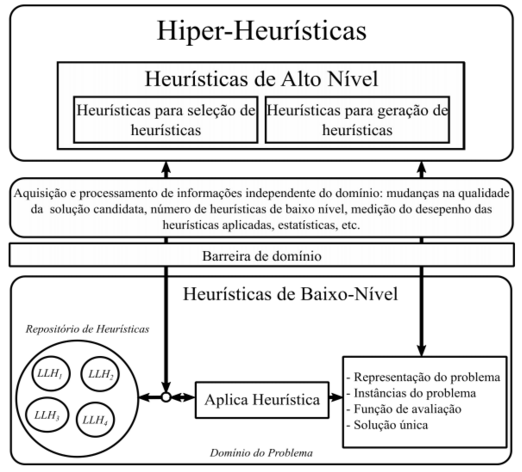
\includegraphics{Imagens/HiperHeuristicas.png}
	\caption{Framework Geral Hiper-Heur�stico. Adaptado de \cite{sabar2015automatic}}
	\label{img:hiperheuristico}
\end{figure}

Como cada inst�ncia ou problema possui um espa�o de busca com diferentes caracter�sticas, os componentes da heur�stica de alto n�vel t�m um grande impacto no desempenho de um \textit{framework} hiper-heur�stico. Esta � uma das raz�es por existir um interesse consider�vel de pesquisa em desenvolver  novos mecanismos de sele��o, assim como diferentes crit�rios de aceita��o \cite{burke2013hyper}. Um bom mecanismo de sele��o deve selecionar a heur�stica mais adequada em um dado momento, para guiar a busca para regi�es promissoras do espa�o de busca. 
Ao utilizar hiper-heur�sticas, espera-se encontrar o m�todo correto ou a sequ�ncia de heur�sticas que mais se adequam a um problema ou inst�ncia ao inv�s de tentar resolver o problema diretamente. Entretanto, um importante objetivo � desenvolver m�todos gen�ricos, que t�m  potencial em produzir solu��es com uma qualidade aceit�vel, utilizando um conjunto de heur�sticas de baixo n�vel f�cil de implementar. As hiper-heur�sticas podem ser classificadas de diversas maneiras. A figura \ref{img:classificacaoHiperHeuristicas} apresenta as poss�veis classifica��es descritas na literatura. 

\begin{figure}[!htb]
	\centering
	\includegraphics{Imagens/ClassificacaoHiperHeuristica.png}
	\caption{Classifica��o Hiper-Heur�sticas.}
	\label{img:classificacaoHiperHeuristicas}
\end{figure}

A primeira classifica��o de hiper-heur�sticas � baseada na sua fonte de conhecimento durante a busca: \textit{Online} � quando a hiper-heur�stica toma decis�es de maneira instant�nea, baseando-se em m�tricas durante sua execu��o, n�o necessitando de treinamento pr�vio. \textit{Offline} necessita de treinamento pr�vio; estes \textit{frameworks}  tomam suas decis�es baseados no que foi aprendido apenas durante o treinamento, sem atualiza��o deste conhecimento. Os \textit{frameworks} classificados como \textit{No-Learning} n�o possuem nenhuma forma de aprendizagem. Outra classifica��o considera como as heur�sticas de baixo n�vel operam sobre as solu��es do problema. As heur�sticas ditas perturbativas realizam pequenas perturba��es nas solu��es gerando novas solu��es. J� heur�sticas construtivas criam solu��es do zero passo a passo e normalmente avaliam cada etapa da constru��o para obter \textit{feedback} sobre o seu desempenho. Uma �ltima  classifica��o, mas n�o menos importante, divide as hiper-heur�sticas de acordo com a  natureza do seu espa�o de busca. As hiper-heur�sticas de sele��o selecionam sequ�ncias de heur�sticas a serem aplicadas para resolver um dado problema ou inst�ncia. J� as hiper-heur�sticas de gera��o operam gerando novas heur�sticas com objetivo de resolver um problema ou inst�ncia.

\subsection{Hiper-Heur�sticas de Sele��o}
\label{Hiper-Heuristicas-Sele��o}

Dentro das hiper-heur�sticas de sele��o, diferentes abordagens/estrat�gias s�o encontradas na literatura:
\begin{itemize}

\item \textit{Random} (R):  Seleciona aleatoriamente as heur�sticas a serem aplicadas.
\item \textit{Choice Function} (CF): Utiliza uma fun��o que leva em considera��o dois fatores: o desempenho das heur�sticas assim como quanto tempo se passou desde a �ltima execu��o de uma heur�stica \cite{burke2013hyper}.
\item \textit{Greedy} (GR): Realiza as escolhas de maneira gulosa levando em considera��o o desempenho das heur�sticas \cite{burke2013hyper}.
\item \textit{Tabu Search Based} (TS): Utiliza uma lista tabu para evitar determinadas heur�sticas que n�o apresentaram bom desempenho \cite{burke2013hyper}.
\item \textit{Multi-Armed Bandit} (MAB): Utiliza uma fun��o baseada em dois componentes: um mede a qualidade de uma determinada heur�stica e est� relacionado � intensifica��o e outro utiliza um intervalo de confian�a baseado no n�mero de vezes que a heur�stica foi aplicada \cite{burke2013hyper}.

\end{itemize}
Al�m de selecionar heur�sticas � necess�rio um crit�rio de aceita��o para definir se uma solu��o gerada por uma heur�stica de baixo n�vel dever� ser aceita ou n�o. Diferentes mecanismos t�m sido propostos na literatura e est�o descritos abaixo:

\begin{itemize}
    \item \textit{All Moves} (AM): Aceita qualquer aplica��o de heur�sticas mesmo que seja sem melhora na solu��o \cite{burke2013hyper}.
    \item \textit{Improvemnt Only} (IO): Aceita apenas aplica��es de heur�stica que melhoraram uma solu��o \cite{burke2013hyper}.
	\item Monte Carlo (MC): Aceita aplica��es de heur�sticas que melhoram uma solu��o e utiliza probabilidades para aceitar aplica��es que n�o melhoram \cite{burke2013hyper}.
	\item \textit{Great Deluge} (GD): Esta estrat�gia estende o algoritmo \textit{Great Deluge} para decidir quando aceitar solu��es geradas pelas heur�sticas \cite{burke2013hyper}.
    
\end{itemize}

\subsection{Hiper-heur�sticas de Gera��o}
\label{Hiper-Heuristicas-Gera�ao}

Estas hiper-Heur�sticas geram novas heur�sticas combinando componentes de heur�sticas existentes. Geralmente se utiliza programa��o gen�tica (GP), ou alguma extens�o como por exemplo evolu��o gramatical \cite{ryan1998grammatical} ou programa��o g�nica \cite{ferreira2006gene}, como hiper-heur�stica para gerar heur�sticas. A pr�xima sub-se��o ir� introduzir o conhecimento necess�rio para a compreens�o da programa��o gen�tica, assim como ir� introduzir evolu��o gramatical, que se trata de um tipo de programa��o gen�tica e que ser� utilizada nesta proposta.

\section{Programa��o Gen�tica (PG)}
\label{subsection:PG}

Programa��o Gen�tica \cite{burke2009exploring} � um ramo da s�ntese de programas que utiliza ideias oriundas da teoria da evolu��o natural para produzir programas. Os principais componentes da computa��o evolucion�ria s�o heran�a (cruzamento/reprodu��o), sele��o e varia��o (muta��o). A heran�a significa que os descendentes  t�m alguma semelhan�a com seus pais, pois quase todo material gen�tico vem dos pais. A sele��o trata de escolher quais pais ir�o se reproduzir para gerar novos descendentes; pais com maior aptid�o tendem a ter maior probabilidade de serem selecionados. Esta press�o de sele��o define quais indiv�duos est�o mais aptos que outros. Varia��o realiza pequenas altera��es em um descendente a fim de criar novo material gen�tico neste indiv�duo e que n�o estava presente em nenhum dos indiv�duos que o geraram. Computa��o evolutiva pode ser pensada como a intera��o destes tr�s componentes. 
Uma popula��o aleat�ria de programas de computador � gerada, e os operadores geneticamente inspirados (cruzamento e muta��o) s�o repetidamente aplicados com objetivo de produzir novos programas de computador. Estes programas s�o avaliados utilizando uma fun��o de \textit{fitness} (normalmente dependente do desempenho obtido pela aplica��o do programa em um problema), que determina quais destes programas s�o mais suscet�veis a sobreviver para gera��es futuras. Os programas com maior aptid�o tem mais chances de serem selecionados para o cruzamento e perpetuarem seus c�digos gen�ticos durante o processo evolutivo. 
Programa��o gen�tica � um m�todo de gera��o de programas sintaticamente v�lidos e a fun��o de \textit{fitness} � utilizada para decidir quais programas s�o mais adequados para o problema.
Na programa��o gen�tica, os programas que comp�em a popula��o s�o tradicionalmente representados utilizando estruturas de �rvore. Existem outras estruturas que podem ser evolu�das, como por exemplo: sequ�ncias lineares de instru��es ou gram�ticas. Nesta proposta ser� utilizada uma representa��o gramatical linear que ser� explicada na se��o \ref{subsubsection:EvolucaoGramatical}.


\section{Evolu��o Gramatical (EG)}
\label{subsubsection:EvolucaoGramatical}

� uma t�cnica relativamente nova de computa��o evolutiva, proposta por Ryan et al. \cite{ryan1998grammatical}, trata-se de uma extens�o da programa��o gen�tica. Assim como na programa��o gen�tica, o principal objetivo � encontrar um programa execut�vel ou trecho de um programa, que obtenha um bom valor de \textit{fitness} para o problema em quest�o. Na maioria dos trabalhos publicados de programa��o gen�tica express�es que representam estruturas de �rvore s�o manipuladas, enquanto na evolu��o gramatical os operadores gen�ticos s�o aplicados em vetores de inteiros que posteriormente s�o mapeados para um programa (ou trecho de programa) atrav�s de uma gram�tica espec�fica. Um dos benef�cios de EG � que este mapeamento generaliza a aplica��o para diferentes linguagens de programa��o.
Ryan el al. \cite{ryan1998grammatical} prop�em uma t�cnica para gerar programas ou fragmentos de programas para qualquer linguagem de programa��o utilizando defini��es BNF. A t�cnica pode ser utilizada para evoluir programas por um processo evolutivo. A evolu��o gramatical adota um mecanismo de mapeamento entre o gen�tipo (indiv�duos codificados em um vetor de inteiros) e o fen�tipo (programas gerados para resolver algum problema). 
A nota��o \textit{Backus Naur Form} (BNF) � a nota��o utilizada para expressar a gram�tica de uma linguagem na forma de regras de produ��o. Uma gram�tica BNF consiste em um conjunto de terminais, os quais s�o itens que podem aparecer na linguagem, por exemplo: +, -, *, / etc e n�o terminais, que podem ser expandidos em um ou mais terminais e n�o terminais. Uma gram�tica pode ser expressada como uma tupla ${N,T,P,S}$, onde $N$ � o conjunto de n�o terminais, $T$ o conjunto de terminais, P um conjunto de regras de produ��o que mapeia os elementos $N$ para $T$; e, por �ltimo, $S$, um s�mbolo de in�cio e que est� contido em $N$.

\begin{center}

$ N = {\langle expr \rangle, \langle op \rangle, \langle pre-op \rangle}$

$ T = {Sin,Cos,Tan,Log,+,-,/,*,X} $

$ S = \langle expr \rangle $

\end{center}

\noindent
E $P$ pode ser representada como:

\begin{Grammar}
\begin{grammar}


<expr> ::=  <expr> <op> <expr> \hspace{9.8cm} (0) 
\alt (<expr> <op> <expr>) \hspace{9.5cm} (1)  
 \alt <pre-op> (<expr>) \hspace{10cm} (2) \alt <var> \hspace{12.1cm} (3) \\\
 
 <op> ::=  + \hspace{12.7cm} (0)   \alt - \hspace{12.9cm} (1)  \alt  /  \hspace{12.85cm} (2) \alt * \hspace{12.85cm} (3) \\
 
 <pre-op> ::= Sin  \hspace{12.4cm} (0) \alt Cos
 \hspace{12.3cm} (1) \alt Tan  \hspace{12.25cm} (2) \alt Cos \hspace{12.3cm} (3) \\
 
 <var> ::= X  \hspace{12.6cm} (0)
 

\end{grammar}

 	\caption{Gram�tica exemplo para demonstrar como decodificar vetores de inteiros em programas de computador.}
	\label{gram:gramatica}
 \end{Grammar}


\begin{table}[htb]
	\centering
	\caption{\textit{Regras de produ��o} e o n�mero de escolhas para cada uma.}
	\label{tab:productionRules}
	\begin{tabular}{|l|l|}
		\hline
		Regra de produ��o & N�mero de escolhas \\ \hline
		$\langle expr \rangle$                        & 4       \\ \hline
		$\langle op \rangle$                         & 4       \\ \hline
		$\langle pre-op \rangle$                         & 4       \\ \hline
		$\langle var \rangle$                          & 1       \\ \hline
	\end{tabular}
\end{table}


Ryan et al. \cite{ryan1998grammatical}  prop�s o uso de um algoritmo gen�tico (AG) para controlar quais escolhas devem ser feitas, permitindo dessa maneira que o AG controle quais regras de produ��o ser�o utilizadas. Um indiv�duo (cromossomo) consiste em um vetor de tamanho vari�vel de valores inteiros que representa o gen�tipo. Para fins de compreens�o o processo de mapeamento de um cromossomo ser� demonstrado utilizando a \autoref{gram:gramatica} apresentada anteriormente nesta se��o. O Algoritmo \ref{alg:pseudocodigogrammar} apresenta o \textit{template} geral dos programas gerados pela \autoref{gram:gramatica}. A express�o $\langle expr \rangle$ apresentada na linha 2 do Algoritmo \ref{alg:pseudocodigogrammar} � substitu�da por express�es matem�ticas que est�o codificadas pelos cromossomos (vetores de inteiros). 

\begin{algorithm}
	\caption{\textit{Template} geral dos algoritmos gerados}
	\label{alg:pseudocodigogrammar}
	float symb(float x) { \\
		a = $\langle expr \rangle$;   \\
		return a;  \\
	}	
\end{algorithm}

\noindent
Suponha o seguinte vetor de inteiros:

\begin{center}
$ [220, 203, 17, 6, 108, 215, 104, 30] $
\end{center}


Este vetor ser� utilizado para mapear o cromossomo (gen�tipo) em um trecho de programa (fen�tipo) utilizando a gram�tica BNF. 
%A express�o n�o terminal $ \langle expr \rangle$ no algoritmo \ref{alg:pseudocodigogrammar} ser� preenchida por um trecho de c�digo que ser� mapeado a partir do cromossomo apresentado. Os passos do mapeamento ser�o descritos a seguir.%
A tabela \autoref{tab:productionRules} resume o n�mero de escolhas associada � cada regra de produ��o da \autoref{gram:gramatica}. Existem 4 op��es de regras de produ��o que podem ser selecionadas para a express�o $ \langle expr \rangle$. Para decidir qual ser� selecionada, o primeiro valor no cromossomo deve ser utilizado. O valor � 220. Devemos realizar o m�dulo deste valor pelo n�mero de escolhas, neste caso 4. Portanto, 220 MOD 4 = 0, o que significa selecionar a primeira op��o: $\langle expr \rangle \langle op \rangle \langle expr \rangle$.

Note que a primeira express�o � novamente $ \langle expr \rangle$ e da mesma maneira devemos obter o pr�ximo valor de inteiro e realizar o m�dulo. O pr�ximo valor inteiro � 203; realizando o modulo de 4, resulta em 3, que portanto seleciona a quarta op��o: $ \langle var \rangle$. Substituindo na express�o anterior, obtemos: $ \langle var \rangle \langle op \rangle \langle expr \rangle$

Nenhuma escolha � necess�ria para a express�o $ \langle var \rangle$, pois existe apenas uma op��o $X$. A express�o pode ser reescrita da seguinte maneira: $X \langle op \rangle \langle expr \rangle$

Neste momento � necess�rio decodificar a express�o n�o terminal $\langle op \rangle$. Obtendo o pr�ximo valor inteiro do cromossomo, temos 17 e para o $ \langle op \rangle$ temos 4 op��es $(+ | - | / | *)$. O resultado de 17 MOD 4  � igual a 1, que significa selecionar:  $-$. Substituindo na express�o, temos: $X  -  \langle expr \rangle$


Novamente � necess�rio fazer uma nova escolha para resolver a express�o n�o terminal $\langle expr \rangle$. O pr�ximo valor do cromossomo � 6 e novamente existem 4 op��es. Realizando o modulo 6 MOD 4, obt�m-se 2, que seleciona $ \langle pre-op \rangle ( \langle expr \rangle)$. Atualizando a express�o, obtemos: $X - \langle pre-op \rangle (\langle expr \rangle)$

Resolvendo a express�o $ \langle pre-op \rangle$, obtemos 108 MOD 4 = 0 que por sua vez seleciona a primeira express�o  terminal $Sin$. Atualizando a express�o, obtemos: $X - Sin (\langle expr \rangle)$

Expandindo $ \langle expr \rangle$, obtemos 215 MOD 4 = 3, que seleciona a express�o n�o terminal $ \langle var \rangle$. J� que para a express�o $ \langle var \rangle$ existe apenas uma op��o, nenhuma escolha � necess�ria e a express�o final decodificada (fen�tipo) �: $X - Sin (X)$

Note que nem todos os genes do cromossomo foram necess�rios para obter o fen�tipo. Nos casos em que isto ocorre, os genes que n�o forem utilizados s�o desconsiderados. Al�m disso, pode ocorrer que um cromossomo n�o tenha genes suficientes para mapear um programa. Neste caso a estrat�gia � reutilizar os genes do cromossomo a partir do primeiro gene. 

Operadores gen�ticos tradicionais (cruzamento e muta��o) tamb�m s�o utilizados na EG. Al�m dos operadores tradicionais outros dois operadores \textit{Prune} e \textit{Duplicate} s�o peculiares � EG e ser�o descritos em seguida:

\begin{itemize}
	\item \textit{Duplicate}: Este operador (dada uma probabilidade) realiza a c�pia de  alguns genes. Os genes duplicados s�o adicionados ap�s a �ltima posi��o do cromossomo. O n�mero de genes a serem duplicados � selecionado de maneira aleat�ria. A motiva��o por tr�s deste operador � que ao duplicar genes ocorre um aumento da presen�a de genes que s�o potencialmente bons, pois pertencem a um indiv�duo com boa aptid�o selecionado pelo operador de sele��o.
	\item \textit{Prune} : Este operador leva em considera��o que nem sempre todos os genes, de um cromossomo, s�o utilizados para decodificar um programa. Dessa maneira (dada uma probabilidade) realiza o truncamento de  cromossomos. O objetivo � diminuir a probabilidade que o operador de cruzamento opere em regi�es dos cromossomos que n�o sejam utilizadas realmente.
\end{itemize}


O Algoritmo \ref{alg:GE} apresenta o pseudoc�digo da evolu��o gramatical (EG). Note que o pseudoc�digo � muito similar a um algoritmo gen�tico simples, exceto pela aplica��o dos operadores \textit{Duplicate} e \textit{Prune} (linhas 10 e 11 do Algoritmo  \ref{alg:GE}) e o processo de decodifica��o e execu��o dos programas descendentes (linhas 13 e 14 do Algoritmo \ref{alg:GE}).


\begin{algorithm}[htb]
	\fontsize{8pt}{10pt}\selectfont
	\caption{Pseudoc�digo da evolu��o gramatical}
	\label{alg:GE}
	\KwIn{AG -- Arquivo da gram�tica}
	\Begin{
		$populacao \gets$ Inicializa��o a popula��o\;
		$programas \gets$ Mapeia $populacao$ para programas utilizando $AG$\;
		Executa os $programas$\;
		Atribui valor de \textit{fitness} para as solu��es  of $populacao$ de acordo com a sa�da obtida pelos respectivos programas decodificados\;
		\While{Condi��o de parada n�o atingida}{
			$pais \gets $ Sele��o de indiv�duos para cruzamento\;
			$descendentes \gets$ Cruzamento $pais$\;
		    Aplica o operator \text{Prune} nas solu��es $descendentes$\;
			Aplica o operador \textit{Duplicate} nas solu��es $descendentes$\;
			Aplica o operador de muta��o nas solu��es $descendentes$\;
			$programas \gets$ Mapeia $descendentes$ para programas utilizando $AG$\;
			Executa $programas$\;
			Atribui valor \textit{fitness} para as solu��es $descendentes$ de acordo com a sa�da obtida pelos respectivos programas decodificados\;
			$populacao \gets$ Realiza substitui��o\;
		}
		\Return{Melhor programa da $populacao$}\;
	}
\end{algorithm}


\section{Programa��o Gen�tica como Hiper-Heur�stica de Gera��o de Heur�sticas}
\label{subsubsection:PGasHH}

Nesta se��o ser�o apresentadas quest�es relativas ao uso de EG como mecanismo de gera��o de heur�sticas. 
Burke et al. \cite{burke2009exploring} descrevem que muitos autores mencionam a melhor adequa��o de programa��o gen�tica, em rela��o a outras t�cnicas de aprendizagem de m�quina, para gerar heur�sticas de maneira autom�tica. Burke et al \cite{burke2009exploring} tamb�m apontam algumas vantagens desta t�cnica:

\begin{itemize}
	\item PG utiliza cromossomos de tamanho vari�vel. Geralmente, n�o se sabe um tamanho �timo para representar heur�sticas de um dado dom�nio de problema.
	\item PG produz estruturas de dados execut�veis. E heur�sticas s�o tipicamente expressadas como programas ou algoritmos.
	\item Facilidade em identificar boas caracter�sticas do dom�nio do problema, afim de definir o conjunto terminal que ser� utilizado pela PG.
	\item Heur�sticas desenvolvidas por humanos podem facilmente ser expressadas na mesma linguagem utilizada para criar o espa�o de busca da PG. O conjunto de fun��es, relevante para o problema pode ser determinado facilmente. E adicionalmente PG pode ser suplementada com uma gram�tica espec�fica.
\end{itemize}

Todas estas vantagens descritas por Burke et al. \cite{burke2009exploring} tamb�m s�o consideradas ao utilizar EG, visto que se trata de uma extens�o de programa��o gen�tica e possui as mesmas caracter�sticas (cromossomo de tamanho vari�vel, produz estruturas execut�veis, etc).
Burke et al. \cite{burke2009exploring} tamb�m mencionam desvantagens, por exemplo: a cada execu��o da programa��o gen�tica � encontrada uma melhor heur�stica que, por se tratar de uma t�cnica estoc�stica, os resultados podem ser distintos em diferentes execu��es. Portanto se fazem necess�rias m�ltiplas execu��es, a fim de se obter um melhor conhecimento da qualidade das heur�sticas que podem ser produzidas. Outra desvantagem � referente � configura��o de par�metros, que normalmente � encontrada via tentativa e erro.

\subsubsection{Abordagem B�sica}

Burke et al. \cite{burke2009exploring} descrevem uma abordagem b�sica para aplicar programa��o gen�tica para gerar heur�sticas:

\begin{enumerate}
	\item Examinar as heur�sticas existentes: Avaliar se as heur�sticas j� propostas para um dado problema podem ser descritas em um \textit{framework} comum. Estas heur�sticas podem ter sido criadas por humanos ou at� mesmo concebidas via outras t�cnicas de aprendizagem. Este passo n�o � trivial, pois envolve o entendimento de um n�mero diverso de heur�sticas existentes, que podem operar de diferentes maneiras. Geralmente heur�sticas desenvolvidas por humanos s�o produtos de anos de pesquisa, portanto uma boa compreens�o das heur�sticas existentes pode ser um trabalho dif�cil. 
	\item Um framework que utilizar� as heur�sticas: neste momento a preocupa��o � em como as heur�sticas ser�o aplicadas para um dado problema. Em geral, os frameworks tendem a ser bem diferentes dependendo do dom�nio do problema. 
	\item Defini��o do conjunto terminal: neste passo a preocupa��o refere-se a vari�veis que expressem o estado do problema. Estas vari�veis ir�o compor os terminais da programa��o gen�tica/evolu��o gramatical. Outros terminais tamb�m podem ser utilizados. Particularmente, constantes aleat�rias podem ser �teis.
	\item Defini��o do conjunto de fun��es: � necess�rio definir como as vari�veis estar�o relacionadas ou combinadas entre si. Estes relacionamentos ir�o compor o conjunto de fun��es da programa��o gen�tica/evolu��o gramatical. 
	\item Identificar uma fun��o de \textit{fitness}: uma fun��o de \textit{fitness} precisa ser identificada para o problema. Geralmente, uma fun��o simples de aptid�o n�o ir� avaliar bem os cromossomos. Introduzir alguns par�metros pode ajudar a encontrar uma mais adequada.
	\item Executar o framework: geralmente ao executar pela primeira vez um framework hiper-heur�stico com programa��o gen�tica, n�o ser�o produzidos bons resultados, devido � escolha dos par�metros. Isto � observado especialmente em casos que o pesquisador � iniciante. Portanto � essencial que as defini��es de par�metros sejam cuidadosamente investigadas.
\end{enumerate}




\section{Considera��es Finais}
\label{ReferencialTeorico:ConsideracoesFinais}


Neste cap�tulo foram apresentados os conceitos que permeiam a �rea de estudo sobre hiper-heur�sticas, tendo sido discutidos os n�veis (alto e baixo) e as classifica��es encontradas na literatura.  Foram discutidas algumas estrat�gias para hiper-heur�sticas de sele��o e gera��o. As hiper-heur�sticas de gera��o foram mais detalhadas, pois esta proposta visa o \textit{design} autom�tico de heur�sticas de alto n�vel. Foram apresentados os conceitos de PG e sua extens�o EG, por se tratarem de estrat�gias comumente utilizadas para o \textit{design} de hiper-heur�sticas de gera��o de heur�sticas. Tamb�m foram discutidas algumas vantagens e desvantagens referentes ao uso de PG para gera��o de heur�sticas, al�m de demonstrar que a EG possui as mesmas caracter�sticas da PG, pois se trata de uma extens�o que utiliza uma gram�tica para gerar os programas. O funcionamento geral da EG foi demonstrado utilizando uma gram�tica exemplo e um vetor de inteiros e, por fim, o pseudoc�digo da evolu��o gramatical foi apresentado. O  \autoref{Problema de Dobramento de Prote�nas} apresenta o problema de dobramento de prote�nas e o \autoref{Metodologia} apresentar� a proposta da aplica��o de EG a este problema.





 	




 



 
















\chapter{Problema de Dobramento de Prote�nas}
\label{Problema de Dobramento de Prote�nas}


\section{Prote�nas}
Prote�nas s�o estruturas b�sicas, essenciais para vida e possuem incont�veis fun��es biol�gicas. Prote�nas s�o sintetizadas pelos ribossomos seguindo um formato provido pelo mensageiro RNA (mRNA). Durante a s�ntese, as prote�nas dobram (enovelam) em uma estrutura tridimensional �nica, conhecida como conforma��o nativa. Este processo � chamado: dobramento de prote�nas (\textit{protein folding}). A fun��o biol�gica de uma prote�na depende da sua estrutura tridimensional.

As prote�nas s�o pol�meros compostos por sequ�ncias de amino�cidos (tamb�m chamados de res�duos) conectados linearmente por liga��es pept�dicas. Cada amino�cido � composto por um �tomo central de carbono ($C\alpha$) conectado a um �tomo de hidrog�nio, um grupo amina, um grupo carboxila e uma cadeia lateral (\textit{side-chain}) a qual confere a cada amino�cido uma fun��o distinta. Uma liga��o pept�dica � formada por dois amino�cidos quando o grupo carboxila de uma mol�cula reage com o grupo amina da outra. Este processo de agrega��o de amino�cidos � conhecido como desidrata��o pois libera uma mol�cula de �gua ($H_2O$) \cite{suzuki1986introduction}. Prote�nas podem ser chamadas de cadeias polipept�dicas. Todos os amino�cidos tem o mesmo \textit{backbone} e se diferem dos outros apenas pela \textit{side-chain}, a qual pode ser um simples �tomo de hidrog�nio ou at� um grupo heteroc�clico complexo. A \textit{side-chain} define as propriedades f�sicas e qu�micas dos amino�cidos de uma prote�na \cite{cox2013lehninger}.

%\subsection{Estrutura hier�rquica e fun��o das prote�nas}

%As prote�nas s�o tradicionalmente descritas em quatro n�veis hier�rquicos de %complexidade \cite{cox2013lehninger}:

%\begin{enumerate}
%	\item Estrutura prim�ria: N�vel de organiza��o simples que visa representar apenas a sequ�ncia de amino�cidos de maneira linear. Representa apenas as liga��es pept�dicas entre os amino�cidos. (Colocar imagem?)
%	\item Estrutura secund�ria: Consiste em arranjos espaciais de regi�es locais de uma prote�na. Existem tr�s estruturas secund�rias importantes $\alpha$-h�lices(PAULING; COREY; BRANSON, 1951a), $\beta$-folhas
%	(PAULING; COREY; BRANSON, 1951b) e turns (dobras) (LEWIS; MOMANY;
%	SCHERAGA, 1973).
%	$\alpha$-h�lices � a forma mais comum de estrutura secund�ria. � uma estrutura semelhante a um bast�o, onde o \textit{backbone} firmemente 
%	helicoide forma a parte interna do bast�o, e as \textit{side-chains} se projetam para fora em uma disposi��o helicoidal(http://labs.icb.ufmg.br/lbcd/grupo1/alfa.html). $\beta$-folhas formada por 2 ou mais segmentos polipept�dicos da mesma mol�cula, ou de mol�culas diferentes, dispostos lateralmente e estabilizados por pontes de hidrog�nio entre os grupos $NH$ e $CO$.  (Ben�tez)
%	\textit{Turns} s�o compostos de tr�s ou quatro amino�cidos e geralmente s�o localizados na superf�cie das prote�nas formando dobras que redirecionam a cadeia polipept�dica para o interior da prote�na. \textit{Turns} permitem que as prote�nas sejam dobradas em estruturas altamente compactas.	As estruturas secund�rias podem ser associadas formando estruturas super secund�rias, chamadas de \textit{motifs} (BRANDEN; TOOZE, 1999; GRIFFITHS
%	et al., 2000; N�LTING, 2006). Os \textit{motifs}  s�o padr�es frequentemente encontrados em estruturas tridimensionais.
	%\item Estrutura terci�ria: Trata do arranjo tridimensional dos amino�cidos que comp�em uma prote�na. Enquanto as estruturas secund�rias s�o estabilizadas por pontes de hidrog�nio, as estruturas terci�rias s�o estabilizadas por itera��es entre \textit{side-chains} hidrof�bicas e pontes de hidrog�nio entre \textit{side-chains} polares. A estrutura terci�ria representa o dobramento de um polipept�deo como resultado das intera��es entre as \textit{side-chains} dos amino�cidos que se encontram em diferentes regi�es da estrutura prim�ria.
%	\item Estrutura quatern�ria: � o n�vel de representa��o mais complexo e descreve o arranjo de duas mais subunidades polipept�dicas dobradas (estruturas terci�rias) no espa�o.
	%A associa��o quatern�ria pode ser entre diferentes tipos de polipept�deos (heterod�mero)
	%ou entre polipept�deos id�nticos (homod�mero). Este n�vel de organiza��o	descreve o n�mero e posi��es relativas de subunidades em prote�nas
	%multim�ricas. A Hemoglobina � um exemplo de prote�na multim�rica, pois � composta de duas c�pias de polipept�deos diferentes que interagem entre si. 
		
%\end{enumerate}

\section{Dobramento de prote�nas}

� o processo em que cada cadeia polipept�dica � transformada em uma estrutura compacta que realiza alguma fun��o biol�gica \cite{grantcharova2001mechanisms}. Estas fun��es incluem controle e regula��o de processos qu�micos essenciais para os organismos vivos \cite{branden1999introduction}. A estrutura tridimensional mais est�vel � chamada de conforma��o nativa e � a qual permite que a prote�na exer�a corretamente sua fun��o biol�gica \cite{lodish2000molecular, pedersen2000algorithms}.

Experimentos conduzidos por Anfinsen et al. \cite{sela1957reductive, anfinsen1972studies, anfinsen1961kinetics}, mostraram que as prote�nas possuem apenas uma conforma��o nativa e que as informa��es essenciais que codificam a estrutura est�o contidas na sequ�ncia de amino�cidos. A conforma��o tridimensional nativa � dada pela estrutura prim�ria (sequ�ncia de amino�cidos) de uma prote�na.

Muitas prote�nas podem desnaturar por modifica��es no ambiente em que est�o inseridas, conforme demonstrado por \cite{sela1957reductive, anfinsen1972studies, anfinsen1961kinetics}. Durante o processo de desnatura��o as prote�nas perdem sua forma nativa (desdobram) e, consequentemente, perdem sua fun��o. O exemplo mais conhecido de desnatura��o proteica � o da clara do ovo. A clara do ovo � composta por �gua e albumina. A albumina � uma prote�na polar, portanto sol�vel em 
�gua. Ao fritar ou cozinhar o ovo, eleva-se a temperatura, levando � desnatura��o da albumina que, mesmo ao retornar � temperatura original, n�o consegue voltar � sua conforma��o nativa. Al�m de se desdobrarem � poss�vel que ocorram erros de dobramento na forma��o das prote�nas causando com que a prote�na n�o exer�a sua fun��o biol�gica corretamente. Estudos tentam identificar causas para os erros de dobramento das prote�nas pois muitas enfermidades s�o causadas pelo mal dobramento de prote�nas como, por exemplo, mal de Alzheimer \cite{hutton2001analysis, selkoe2001clearing}, alguns tipos de c�ncer \cite{bell2002p53, dawson2003n, ishimaru2003fibrillar}, fibrose c�stica \cite{thomas1992altered}, arteriosclerose
\cite{ursini2002atherosclerosis}, mal de Parkinson \cite{mcnaught2001failure}, entre outras. 
Portanto, entender como o processo de dobramento de prote�nas ocorre � de fundamental import�ncia. Um dos objetivos comuns das ci�ncias biol�gicas � caracterizar funcionalmente sequ�ncias de prote�nas atrav�s da resolu��o de suas conforma��es nativas \cite{eswar2003tools}. Varias �reas da ci�ncia, tais como Biologia, Medicina, Qu�mica Org�nica, realizam diferentes estudos das prote�nas. Muitos destes estudos s�o voltados para o processo de dobramento das prote�nas que pode sofrer altera��es: tanto em como a conforma��o estar� disposta no espa�o, como ela estar� agrupada e sobre sua m� forma��o. Isto � muito relevante para estudos que visam � produ��o de medicamentos, suplementos alimentares, t�cnicas que manipulam o DNA, ou para forma��o de novos compostos proteicos sint�ticos em laborat�rio \cite{devlin1998manual}. � importante mencionar que apesar do avan�o na grande quantidade de prote�nas que se tem conhecimento por conta de projetos de sequenciamento gen�mico, apenas uma pequena fra��o de estruturas tridimensionais � conhecida.

A cristalografia de raios-X e espectroscopia de RNM s�o os m�todos experimentais mais poderosos para o estudo da estruturas de prote�nas \cite{ilari2008protein} \cite{gobl2012application}. Entretanto estes m�todos s�o altamente custosos tanto em esfor�os computacionais, de tempo e financeiros, e est�o dispon�veis apenas para algumas institui��es.


Embora o conceito de dobramento de prote�nas tenha surgido da �rea de biologia molecular, este problema � um problema interdisciplinar, o qual requer apoio de muitas �reas do conhecimento, e � considerado como um dos desafios atuais mais importantes da biologia e bioinform�tica \cite{nicosia2008generalized}. 

Na biologia computacional existem dois problemas que tratam sobre o dobramento de prote�nas. S�o eles: problema de predi��o estrutura de prote�nas (ou PSP - \textit{Protein Structure Prediction}), que trata de predizer a estrutura tridimensional (conforma��o) a partir de sua sequ�ncia (estrutura prim�ria); e o problema de dobramento de prote�nas (PDP ou PFP - \textit{Protein Folding Problem}), o qual trata da determina��o dos passos/eventos que conduzem o dobramento a partir da estrutura prim�ria at� a conforma��o nativa \cite{lopes2008evolutionary}. Por�m, na literatura, � encontrado ambos os termos sendo utilizados sem nenhuma distin��o, normalmente se referindo apenas ao primeiro problema \cite{lopes2008evolutionary}.  

A ci�ncia da computa��o desempenha um papel importante nisto, propondo e desenvolvendo modelos e solu��es computacionais para o estudo de ambos os problemas PSP e PDP \cite{lopes2008evolutionary}. Muitas estrat�gias computacionais descrevem modelos de predi��o de estruturas de prote�nas com diferentes n�veis de detalhamento e complexidade mas que permitem uma representa��o fidedigna da estrutura tridimensional, sem perda de viabilidade computacional \cite{benitez2015algoritmo}. Dessa maneira  evita-se a obrigatoriedade do uso de m�todos caros, aumentando a competitividade e auxiliando na consolida��o de centros de pesquisa que desenvolvem estudos nesta �rea \cite{dill2000polymer}.

Acredita-se que a conforma��o nativa de uma prote�na � a sua estrutura mais est�vel, adquirindo um estado de energia livre m�nima, o que gerou a chamada hip�tese da termodin�mica \cite{pedersen2000algorithms}. Os modelos de predi��o de estruturas normalmente s�o baseados nas leis da termodin�mica onde o problema � modelado como um problema de minimiza��o da energia livre a respeito das poss�veis conforma��es que uma prote�na pode assumir \cite{benitez2015algoritmo}. A minimiza��o da energia livre � assumida como o principal fator para a forma��o da estrutura da prote�na. Portanto, a conforma��o nativa de uma prote�na � dada por aquela que possuir o menor valor de energia livre.

Segundo \cite{pedersen2000algorithms}, um modelo computacional deve possuir algumas caracter�sticas:

\begin{itemize}
	\item Um conjunto de entidades que representam os �tomos e as liga��es entre eles. 
	\item Regras que definem as poss�veis conforma��es.
	\item Uma fun��o que seja computacionalmente fact�vel, para calcular a energia livre das poss�veis conforma��es.
\end{itemize}

A pr�xima subse��o ir� discorrer sobre alguns modelos de representa��o de estruturas de prote�nas.

\section{Modelos de Representa��o de Prote�nas}

Em suma existem duas classes de modelos de representa��o de estruturas de prote�nas: anal�tico (tamb�m conhecido como \textit{all atom}) e discreto (chamado tamb�m de \textit{coarse-grained}). Os modelos anal�ticos possuem uma descri��o detalhada da estrutura tridimensional incluindo informa��es de todos os �tomos que constituem uma prote�na. J� os modelos discretos descrevem as prote�nas com um n�vel bastante reduzido de detalhes. Os modelos discretos recentemente ganharam maior interesse, por conta de dois fatores: a simula��o de modelos anal�ticos nem sempre � computacionalmente poss�vel e modelos discretos possibilitam simula��es biologicamente relevantes com melhor aproveitamento  computacional \cite{benitez2015algoritmo}. Embora simula��es utilizando modelos discretos ainda n�o possam ser consideradas t�o preditivas quanto simula��es anal�ticas, avan�os not�veis t�m: sido alcan�ados, referente ao uso de metodologias mais rigorosas e cria��o de algoritmos para melhor explorar o espa�o de busca \cite{tozzini2005coarse}. Esta proposta ir� descrever apenas os modelos discretos pois visa a utiliza��o do modelo hidrof�bico polar (HP) 2D.

\subsection{Modelos Discretos}

Os modelos computacionais mais simples s�o os conhecidos como modelos de grade (\textit{lattice models}). Estes modelos consideram as estruturas de prote�nas como um colar de esferas posicionado em uma grade. O grau de liberdade dos movimentos � restrito � estrutura da grade, que pode ser 2D (plano) ou 3D (espacial). Conforma��es v�lidas s�o aquelas que os amino�cidos adjacentes na sequ�ncia tamb�m s�o adjacentes na grade e cada amino�cido ocupe uma posi��o distinta na grade. Muitos modelos de grade t�m sido propostos e aplicados ao PDP. Os modelos 2D-HP e 3D-HP s�o exemplos de modelos de grade.

\subsubsection{Modelo Hidrof�bico-Polar HP}
\label{subsubsection:modeloHP}

 No modelo HP os amino�cidos s�o classificados em 2 tipos: Hidrof�licos (Polar) e Hidrof�bico. Consequentemente, uma prote�na � representada por uma \textit{string} de caracteres definida por um alfabeto bin�rio $\{H,P\}$. Este modelo considera que as intera��es entre amino�cidos hidrof�bicos (H) representam a contribui��o mais importante para a energia livre de uma prote�na. Portanto existe uma rela��o inversamente proporcional: quanto maior for a quantidade de intera��es hidrof�bicas (H-H), menor ser� a energia livre de uma prote�na. Uma intera��o hidrof�bica (tamb�m conhecida como contato hidrof�bico) � definida como um par de amino�cidos do tipo H-H que n�o sejam consecutivos na sequ�ncia mas sejam adjacentes na grade.
 Como dito anteriormente, uma conforma��o � dita v�lida quando nenhuma posi��o da grade � ocupada por mais que um amino�cido. Conforma��es inv�lidas possuem colis�es entre os amino�cidos. Dada uma conforma��o v�lida para o modelo HP e $n$ o n�mero de intera��es hidrof�bicas, a energia da conforma��o pode ser facilmente calculada utilizando a equa��o \ref{equation:energyHp}: 
 
 
 \begin{align}
 \label{equation:energyHp}
  E(c) = n. (-1) 
 \
 \end{align}

 
 Quando uma prote�na � dobrada na sua conforma��o nativa, os amino�cidos hidrof�bicos tendem a se agrupar no interior da estrutura, protegidos por amino�cidos polares posicionados no exterior. Dessa maneira, um n�cleo hidrof�bico � formado em prote�nas dobradas \cite{benitez2015algoritmo}. 
 Embora simples, a estrat�gia computacional de buscar uma solu��o para o PDP utilizando modelo HP � considerada como um problema $NP$-completo \cite{atkins1999intractability, berger1998protein, crescenzi1998complexity}. O espa�o de busca do modelo HP possui algumas caracter�sticas mencionadas na literatura \cite{bastolla1997testing, berger1998protein, crescenzi1998complexity, krasnogor1999protein, vendruscolo2000can} :
 
 \begin{itemize}
	\item Elevada degeneresc�ncia.
	\item Espa�o de busca multimodal.
	\item Muitas regi�es com conforma��es inv�lidas.
 \end{itemize}
 
 A figura \ref{fig:exemploModeloHP} apresenta um exemplo para os modelos HP (2D e 3D). Os pontos pretos s�o amino�cidos do tipo H e os brancos s�o amino�cidos do tipo P. As linhas pontilhadas representam as intera��es hidrof�bicas.
 
 \begin{figure}[!htb]
 	\centering
 	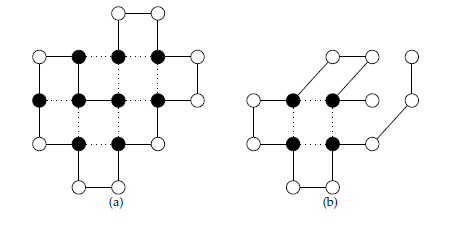
\includegraphics[scale=.9]{modeloHP/modeloHPExemplo.png}
 	\caption{Exemplos de representa��o de prote�nas utilizando os modelos HP 2D-HP (a) e 3D-HP (b). \\ Fonte: Adaptado de \cite{benitez2015algoritmo}}
 	\label{fig:exemploModeloHP}
 \end{figure}
 

Diversos trabalhos aplicam algoritmos evolucion�rios e bio-inspirados ao problema de dobramento de prote�nas utilizando o modelo HP. Uma decis�o comum a todos trabalhos que utilizam o modelo HP � a de como representar as vari�veis de entrada. Na literatura � poss�vel encontrar basicamente tr�s representa��es \cite{krasnogor1999protein, lopes2008evolutionary}: 

\begin{itemize}
	 \item Coordenadas cartesianas: Este m�todo  representa a posi��o de cada amino�cido utilizando suas coordenadas espaciais (x,y) no plano cartesiano 2D ou (x,y,z) no plano cartesiano 3D. Geralmente, sua utiliza��o n�o � adequada para algoritmos baseados em popula��o, pois estruturas id�nticas ou semelhantes podem ter coordenadas totalmente diferentes  \cite{benitez2015algoritmo}; 
	 \item Coordenadas internas: Nesta representa��o as conforma��es s�o representadas por conjuntos de movimentos que ditam como a estrutura final ir� se parecer. Esta representa��o � a mais utilizada em abordagens com algoritmos evolucion�rios para o PDP \cite{benitez2015algoritmo}. Existem duas possibilidades de se representar conforma��es utilizando coordenadas internas:
	 \begin{itemize}
		\item Coordenadas absolutas: Este tipo de coordenada � baseado na orienta��o do eixo da grade onde a conforma��o esta contida. No caso de uma grade bidimensional os poss�veis movimentos s�o: $\{N,S,L,O\}$ ou norte,sul,leste e oeste. J� em uma grade 3D os poss�veis movimentos s�o: $\{N,S,L,O,F,T\}$ que correspondem aos mesmos movimentos no caso 2D por�m com dois movimentos a mais: para frente e para tr�s.
		\item Coordenadas relativas: Este tipo de representa��o define a posi��o de cada amino�cido da cadeia em rela��o ao movimento do seu predecessor. O conjunto de movimentos poss�veis para a grade 2D � definido por $\{F,E,D\}$, que correspondem aos movimentos: frente (continuar no mesmo sentindo do amino�cido anterior), � esquerda e � direita. Em um cubo 3D, os poss�veis movimentos s�o $\{F,E,D,C,B,\}$, possuindo dois movimentos a mais: para cima e para baixo. 
	 \end{itemize}
	 \item Matriz de dist�ncias: descreve a conforma��o de uma prote�na atrav�s de uma matriz quadrada que representa a dist�ncia entre os amino�cidos. Este tipo de representa��o � raramente utilizado na literatura \cite{benitez2015algoritmo}.
\end{itemize}
 
 
 
 \subsubsection{Outros Modelos}


Al�m do modelo HP, outros modelos simples em grade s�o utilizados para representar a estrutura de prote�nas em outros estudos encontrados na literatura. Por exemplo:

\begin{itemize}
	\item Modelo PH (\textit{Perturbed Homopolymer}): Proposto por Shakhnovich et al. \cite{shakhnovich1993engineering}, as rea��es entre amino�cidos hidrof�bicos n�o s�o levadas em considera��o, mas as intera��es entre amino�cidos do mesmo tipo s�o favorecidas, ou seja, H-H e P-P, desfavorecendo liga��es H-P \cite{benitez2015algoritmo}.
	\item Modelo LPE (\textit{Lattice Polymer Embedding}): Modelo proposto por Unger e Moult \cite{unger1993finding}. A modelagem � feita a partir de uma sequ�ncia de amino�cidos, A = $a_1,...a_n$ atrelada a uma grade c�bica. Cada amino�cido possui um coeficiente de afinidade, definido para cada par $a_i,a_j (c(a_i,a_j))$. O objetivo da fun��o de energia � minimizar o produto dos coeficientes pela dist�ncia entre os amino�cidos \cite{benitez2015algoritmo}.
	\item Modelo HP-TSSC (\textit{Hydrophobic-Polar Tangent Spheres Side Chain Model}): este modelo
	proposto por Hart et al. \cite{hart1997lattice} � baseado no modelo HP, por�m n�o
	utiliza uma grade. Neste modelo a prote�na � modelada via um grafo tridimensional, onde a cadeia lateral e o \textit{backbone}
	de cada amino�cido s�o esferas de mesmo raio \cite{benitez2015algoritmo}.
	\item Modelo CGE (\textit{Charged Graph Embedding}): Modelo descrito por Ngo et al. \cite{ngo1994protein}. Neste modelo, uma carga (\textit{charge}) � atribu�da a cada
	res�duo. Entretanto, as conforma��es permitidas n�o s�o realistas \cite{benitez2015algoritmo}. 
	\item Modelo HPNX: modelo proposto por Bornberg-Bauer \cite{bornberg1997chain}. Divide
	os 20 amino�cidos em 3 classes: hidrof�bicos (H), positivos (P), negativos
	(N) e neutros (X). Este modelo, assim como o modelo HP, utiliza uma grade. Intera��es entre amino�cidos hidrof�bicos (H-H) representam
	intera��es de atra��o e diminuem a energia da conforma��o em 4,0,
	as intera��es entre positivos (P-P) e negativos (N-N) representam intera��es de repuls�o e aumentam a energia livre em 1,0 e as intera��es entre N e P decrescem a energia em 1,0. O objetivo tamb�m consiste em minimizar a energia livre. Da mesma maneira que o modelo HP, quanto mais intera��es hidrof�bicas melhor ser� o dobramento. Por�m este modelo n�o desconsidera o valor das demais intera��es \cite{benitez2015algoritmo}.
	\item Modelo HP-helicoidal (Helical-HP): este modelo proposto por Thomas e Dill \cite{thomas1993local} considera apenas uma grade bidimensional e inclui dois tipos de intera��o: intera��es n�o-locais atrav�s de energia de contatos hidrof�bicos e intera��es locais representadas por uma tend�ncia � forma��o de a-h�lices (chamada de propens�o h�lica) \cite{benitez2015algoritmo}.
	\item Modelo \textit{off-lattice} AB: este modelo proposto por Stillinger et al. \cite{stillinger1993toy} divide os amino�cidos em duas classes de acordo com sua polaridade: Hidrof�bicos (A) e Hidrof�licos (ou polares  B). Inicialmente, este modelo foi aplicado em duas dimens�es (2D AB \textit{off-lattice}) e posteriormente aplicado para tr�s dimens�es (3D AB \textit{off-lattice}). Os amino�cidos n�o consecutivos interagem atrav�s de um potencial modificado de Lennard-Jones. Os �ngulos de tors�o entre liga��es sucessivas tamb�m contribuem no c�lculo da fun��o de energia \cite{benitez2015algoritmo}.
	
\end{itemize}




\section{Considera��es Finais}
\label{Problema de Dobramento de Prote�nas:Consideracoes Finais}

Neste cap�tulo o problema de dobramento de prote�nas foi apresentado e sua import�ncia para biol�gica computacional, qu�mica org�nica e medicina. Tamb�m foi mencionado que existem diversos modelos para representar estruturas de prote�nas. Cada modelo tem suas peculiaridades e considera intera��es diferentes. N�o existe um modelo que represente de maneira real o dobramento de prote�nas, pois se trata de um processo ainda n�o completamente compreendido pelos cientistas e pesquisadores. Os modelos propostos tem diferentes n�veis de detalhe e complexidade. O modelo mais simples � o HP mas apesar da sua simplicidade se apresenta como um problema $NP$-completo. O modelo HP ser� utilizado nesta proposta por conta de sua simplicidade de implementa��o, assim como o baixo custo computacional para realizar simula��es do c�lculo de energia. Utilizando o modelo HP diferentes maneiras de representar as vari�veis existem. Nesta proposta iremos utilizar a representa��o relativa pois � mencionado na literatura que esta tem uma maior capacidade de guiar algoritmos de busca a melhores resultados.



 


\chapter{Trabalhos Relacionados}
\label{Trabalhos Relacionados}

Este cap�tulo ir� apresentar alguns trabalhados relacionados com a presente proposta. Ser�o apresentados trabalhos que buscam construir/adaptar estrat�gicas heur�sticas para encontrar melhores solu��es ao PDP utilizando o modelo HP. Tamb�m ser�o apresentados alguns trabalhos que utilizam t�cnicas de programa��o gen�tica para gerar heur�sticas para diferentes problemas.


%Tamb�m ser� apresentado um trabalho que trata do \textit{design} autom�tico de heur�sticas de alto n�vel para um \textit{framework}  hiper-heur�stico aplicado a problemas de \textit{benchmark} disponibilizados pelo \textit{software} HyFlex \cite{ochoa2012hyflex}.

Unger e Moult em seu trabalho de grande influ�ncia \cite{unger1993genetic} foram percussores ao aplicar um algoritmo gen�tico ao PDP com o modelo HP, utilizando operadores de cruzamento e muta��o aprimorados. Os resultados apresentados superam um n�mero significativo de estrat�gias tradicionais anteriores que utilizam m�todos Monte Carlo para explorar as conforma��es. 

Um algoritmo gen�tico multi mem�tico foi proposto por Krasnogor et al. \cite{krasnogor2002multimeme}. Esta estrat�gia combina um algoritmo gen�tico e buscas locais selecionando a busca local que mais se adequar com a inst�ncia (sequ�ncia) sendo otimizada. Mais tarde este trabalho foi aprimorado com um estrategia \text{fuzzy} para as buscas locais, dessa maneira produzindo melhores resultados para o PDP.

Em \cite{hsu2003growth}, os autores utilizam um algoritmo de crescimento de cadeia, chamado \textit{pruned-enriched Rosenbluth method} (PERM). Esta estrat�gia se baseia em iterativamente construir uma conforma��o adicionando os amino�cidos um a um. 

A otimiza��o de col�nia de formigas tamb�m foi aplicada para o PDP nos trabalhos \cite{shmygelska2002ant,shmygelska2003improved}. Estas abordagens utilizam formigas artificiais com objetivo de construir as conforma��es para o modelo HP. Uma busca local tamb�m foi introduzida com objetivo de melhorar e manter a qualidade das solu��es. 

Santana el al. \cite{santanna2008} prop�em a aplica��o de diferentes algoritmos de estima��o de distribui��o (AED) para o PDP. Os AEDs s�o capazes de aprender a explorar as regularidades do espa�o de busca utilizando modelos de depend�ncia probabil�sticos. Os autores compararam os resultados com as abordagens descritas anteriormente neste cap�tulo e constataram que a sua abordagem conseguiu atingir os valores �timos para v�rias sequ�ncias de amino�cidos.

O estudo desenvolvido por Lin et al. \cite{lin2011protein} utiliza um algoritmo gen�tico h�brido combinando um operador de muta��o baseado na otimiza��o por exame de part�culas. Os resultados apresentados por Lin et al. se mostraram superiores aos apresentados por outros estudos, da �poca, que utilizam algoritmos evolutivos. Este trabalho tamb�m utiliza operadores de buscas locais que ser�o utilizados como heur�sticas de baixo n�vel na presente proposta. 


Cust�dio et al. \cite{custodio2014multiple} desenvolveram um metodologia que consistiu modificar um algoritmo gen�tico para selecionar os operadores de cruzamento e muta��o de maneira din�mica. Al�m disso, utilizar�o um mecanismo baseado em \textit{crowding}  para manter a diversidade durante o processo de busca. Este trabalho apresentou bons resultados em rela��o a outros estudos que exploram algoritmos evolutivos. Os operadores gen�ticos utilizados deste trabalho tamb�m ser�o implementados como heur�sticas de baixo n�vel nesta proposta. 


Louren�o el al. \cite{lourencco2012evolving} desenvolveram uma estrat�gia de gera��o e \textit{tuning} autom�tica    


O trabalho desenvolvido por Sabar et al. \cite{sabar2014automatic} prop�e uma estrat�gia, utilizando \text{Gene Expression Programming} (GEP), de gera��o de heur�sticas de alto n�vel para um \textit {framework} hiper-heur�stico aplicado a diversos problemas de \textit{benchmark} contidos no \text{framework} HyFlex \cite{ochoa2012hyflex}. Este trabalho se difere dos apresentados anteriormente pois foi aplicado a dom�nios de problemas diferentes do PDP. Este trabalho motivou a presente proposta pois os resultados apresentados se mostraram promissores. A aplica��o de uma vertente de programa��o gen�tica para gera��o de heur�sticas tem uma maior capacidade de explorar espa�os de busca complexos (com muitos m�nimos locais) e com muitas restri��es.



%TODO: Melhorar essa parte em conjunto com as consideracoes finais
A presente proposta visa aplicar evolu��o gramatical (EG) pois apesar de possuir as mesmas caracter�sticas da GEP ela torna mais amig�vel a manipula��o dos indiv�duos. Isto ocorre pelo fato de represent�-los utilizando vetores de inteiros enquanto a GEP utiliza vetores de strings para representa��o. Dessa maneira, a EG facilita a manipula��o dos indiv�duos por operadores gen�ticos (cruzamento de muta��o). A principal diferen�a entre esta proposta e os outros trabalhos relacionados \cite{santanna2008,shmygelska2002ant,shmygelska2003improved,hsu2003growth, krasnogor2002multimeme,krasnogor2002multimeme,unger1993genetic} � que este ir� trabalhar em um n�vel acima: gerando heur�sticas de alto n�vel para um \textit{framework} hiper heur�stico que ser� aplicado ao PDP enquanto os outros trabalham aplicando meta-heur�sticas diretamente ao PDP. 



\section{Considera��es Finais}
\label{TrabalhosRelacionados:ConsideracoesFinais}

%TODO: Melhorar essa parte
Neste cap�tulo foram discutidos alguns estudos que utilizam algoritmos de busca para explorar o espa�o de busca do PDP utilizando o modelo HP. Tamb�m foram discutidos trabalhos que aplicam PG como hiper-heur�stica de gera��o de heur�sticas. Foram mencionadas diferentes estrat�gias de busca para o PDP algumas destas estrategias servem de base para alguns componentes que esta proposta possui. Os operadores gen�ticos utilizados \cite{custodio2014multiple} e \cite{lin2011protein} servir�o de mat�ria prima para as heur�sticas de baixo n�vel desta proposta. J� os resultados apresentados pelo trabalho desenvolvido por Sabar et al. \cite{sabar2015automatic}, o qual (GEP) como heur�stica de gera��o de heur�sticas, instiga a aplica��o de uma estrat�gia utilizando 

\chapter{Metodologia}
\label{Metodologia}
Neste cap�tulo ser� apresentada a metodologia para aplica��o da EG para gera��o de heur�sticas de alto n�vel para um \textit{framework} hiper-heur�stico  para o problema de dobramento de prote�nas. Esta proposta � baseada no trabalho desenvolvido por Sabar et al. \cite{sabar2015automatic}, o qual  utilizou GEP (\textit{gene expression programming}) com objetivo de gerar os componentes de um \textit{framework} hiper-heur�stico para diversos dom�nios de problemas. Os testes de generalidade realizados por Sabar, utilizando os 6 dom�nios providos pelo \textit{framework} hiper-heur�stico HyFlex, apresentaram bons resultados em rela��o �s outras estrat�gias hiper-heur�sticas do estado da arte. Nesta proposta pretende-se utilizar EG ao inv�s de GEP e aplicar ao PDP utilizando o modelo HP-2D. A representa��o de coordenadas relativas, descrita na subse��o \ref{subsubsection:modeloHP}, ser� utilizada pois segundo o estudo realizado por Krasnogor et al. \cite{krasnogor1999protein} apresentam um maior potencial em conduzir os algoritmos a resultados melhores. Para representar as solu��es ao problema PDP utilizando coordenadas relativas um esquema de codifica��o precisa ser definido. Esta representa��o utiliza um conjunto de movimentos para cada amino�cido baseado no seu predecessor. Os movimentos permitidos para o modelo HP-2D s�o: frente (F), esquerda(E) e direita(D). Dessa maneira, foi definido o seguinte esquema de codifica��o utilizando valores inteiros F->0, E->1 e D->2. Portanto o alfabeto utilizado para representar as solu��es � definido como $\{0,1,2\}$. Como mencionado anteriormente, um \textit{framework} hiper-heur�stico possui dois n�veis: alto (\textit{high-level heuristics}) e baixo (\textit{low-level heuristics}). Nesta proposta as heur�sticas de alto n�vel s�o compostas por: um mecanismo de sele��o e um crit�rio de aceita��o. J� as heur�sticas de baixo n�vel consistem em um conjunto de heur�sticas, selecionadas de estudos anteriores, um mecanismo de mem�ria e uma fun��o de \textit{fitness}. 

\section{\textit{Heur�sticas de alto n�vel}}
\label{sec:highlevelheuristics}
  A presente proposta projeta a gera��o \textit{online} dos componentes de uma heur�stica de alto n�vel (mecanismo de sele��o e crit�rio de aceita��o) para um \textit{framework} hiper-heur�stico. A figura \ref{fig:proposedFramework} apresenta o \textit{framework} proposto.

 \begin{figure}[!htb]
 	\centering
 	\includegraphics[scale=.98]{HH/proposedFramework.png}
 	\caption{\textit{Framework} proposto. \\ Fonte: Adaptado de \cite{sabar2014automatic}}
 	\label{fig:proposedFramework}
 \end{figure}
 
  
    
	Heur�sticas de alto n�vel geralmente levam em considera��o uma ou mais informa��es referentes ao hist�rico das aplica��es das heur�sticas de baixo n�vel para tomar suas decis�es. Tradicionalmente, informa��es tais como desempenho (capacidade de melhorar solu��es), tempo (desde a �ltima aplica��o de uma dada heur�stica) e intervalo de confian�a (no caso de estrat�gias que utilizam MAB) s�o utilizadas como base de conhecimento. Sabar et al. \cite{sabar2015automatic} prop�em a utiliza��o de v�rios crit�rios para avaliar as heur�sticas de baixo n�vel. A raz�o disto se d� pelo fato de que cada crit�rio ir� favorecer a sele��o de uma heur�stica de baixo n�vel a partir de uma perspectiva diferente. Por exemplo, algumas heur�sticas de baixo n�vel podem ter bom desempenho apenas no in�cio da busca, enquanto outras podem obter melhores resultados apenas ao final. Estes crit�rios propostos por Sabar et al. \cite{sabar2015automatic} cont�m estat�sticas referente � aplica��es das heur�sticas de baixo n�vel e s�o gen�ricos o suficiente para serem aplicados ao PDP. Os crit�rios propostos por Sabar et al. \cite{sabar2015automatic} s�o detalhados em seguida:
	
	
\begin{itemize}
	\item RC (\textit{Reward Credit}): Representa a recompensa que uma determinada heur�stica de baixo n�vel deve receber baseado no seu desempenho durante o processo de busca. Quando a i-�sima heur�stica � aplicada, a melhoria para a solu��o � computada. O c�lculo da melhoria � dado por: $M(i) = (|f1 -f2|/f1) *100$ se $f2$< $f1$, onde $f1$ � a qualidade da solu��o corrente e $f2$ � a qualidade da solu��o resultante ap�s a aplica��o da i-�sima heur�stica. 
	A melhoria obtida � salva em uma janela deslizante (FIFO) de tamanho W. O cr�dito de qualquer heur�stica de baixo n�vel � ent�o atribu�do como o m�ximo valor na janela deslizante correspondente. A ideia por tr�s deste crit�rio �: heur�sticas de baixo n�vel que n�o s�o usadas com frequ�ncia mas que alteram a solu��o com grandes melhorias tendem a ter mais prefer�ncia do que aquelas que geram pequenas melhorias. Portanto as heur�sticas que trazem frequentes, mas pequenas melhorias ir�o ter menos probabilidade de serem selecionadas.
	\item $C_{best}$: N�mero de vezes que a i-�sima heur�stica de baixo n�vel atualizou a melhor solu��o conhecida. Este crit�rio favorece as heur�sticas de baixo n�vel que obtiveram �xito em melhorar a melhor solu��o conhecida at� o momento. Este crit�rio � �til para sistematicamente melhorar o atual m�nimo local.
	\item $C_{current}$: N�mero de vezes que a i-�sima heur�stica de baixo n�vel atualizou a solu��o atual. Este crit�rio favorece as heur�sticas de baixo n�vel que obt�m �xito em atualizar a solu��o corrente. Este crit�rio serve para deixar a busca concentrada pr�xima � solu��o corrente.
	\item $C_{accept}$: N�mero de vezes que a solu��o gerada pela i-�sima heur�stica de baixo n�vel foi aceita pelo crit�rio de aceita��o. Ir� favorecer heur�sticas de baixo n�vel que podem ajudar a escapar de um m�nimo local.
	\item $C_{ava}$: A m�dia de melhorias anteriores da i-�sima heur�stica de baixo n�vel durante o progresso da busca. Este crit�rio favorece heur�sticas de baixo n�vel que realizaram grandes melhorias em m�dia.
	\item $C_r$: O n�mero de vezes que a i-�sima heur�stica de baixo n�vel foi classificada como primeira.  
\end{itemize} 

	Da mesma maneira Sabar et al. \cite{sabar2015automatic} prop�em o uso de dados referentes ao hist�rico de aplica��es das heur�sticas de baixo n�vel para compor crit�rios de aceita��o que ir�o definir um limites para aceitar solu��es com qualidade inferior. Dessa forma, um conjunto de fatores tamb�m foi proposto e ser� detalhado em seguida:
	
	
	 \begin{itemize}
	 	\item Delta: A diferen�a da qualidade entre  solu��o corrente e a solu��o descendente.
	 	\item PF: A qualidade da solu��o anterior.
	 	\item CF: A qualidade da solu��o atual.
	 	\item CI: Itera��o corrente.
	 	\item TI: N�mero de itera��es.
	 \end{itemize}
	 
	 
	Estes dados ser�o inicializados com valores neutros dessa maneira evitando qualquer comportamento tendencioso. Os dados  ser�o atualizados conforme o desempenho e estado das heur�sticas de baixo n�vel durante o progresso da busca.   

	Utilizando estes dados estat�sticos e um conjunto de fun��es matem�ticas simples, tais como soma, subtra��o, multiplica��o e divis�o, uma gram�tica foi desenvolvida para suportar a gera��o das heur�sticas de alto n�vel. A gram�tica desenvolvida para gerar mecanismos de sele��o e crit�rios de aceita��o � apresentada na \autoref{grammar:proposedGrammar}. 
	

	
	% e combinados com fun��es matem�ticas simples comp�em a \autoref{grammar:proposedGrammar}

 
 
 % TODO: Talvez levar isso para se�ao de EG
 %Como mencionado na subse��o \ref{subsubsection:EvolucaoGramatical}, a EG utiliza vetores de valores inteiros com tamanho vari�vel para representar seus indiv�duos. Dessa maneira, a EG junta as vantagens tanto de algoritmos gen�ticos como de programa��o gen�tica para evoluir popula��es de programas de computador.
 
 
 

 
 \begin{Grammar}
 	\begin{grammar}
 		<hh-selection> ::= <selection-mechanism> <acceptance-criterion> 
 		
 		<selection-mechanism> :==  <selection-terminal>   
 		\alt <selection-mechanism> <math-function> <selection-mechanism> 
 		\alt (<selection-mechanism> <math-function> <selection-mechanism>) 
 		
 		<selection-terminal> :== 
 		RC 
 		| Cbest 
 		| Ccurrent 
 		| Caccept 
 		| Cava 
 		| Cr
 		
 		<math-function> :== + 
 		| - 
 		| * 
 		| \%
 		
 		<acceptance-criterion> ::== <acceptance-terminal> 
 		\alt <acceptance-criterion> <math-function>
 		<acceptance-criterion>
 		\alt (<acceptance-criterion>  <math-function> <acceptance-criterion>) 
 		
 		<acceptance-terminal> :== PF | CF | CI | TI
 		
 	%	<acceptance-function> :== + | - | * | \% | $e^x$
 		
 		
 	\end{grammar}
 	\caption{Gram�tica definida para gerar  heur�sticas de alto n�vel}
 	\label{grammar:proposedGrammar}
 \end{Grammar}
 
 
 
 %O conjunto de fun��es e terminais apresentado na gram�tica \ref{grammar:proposedGrammar} foi desenvolvido baseado nos conjuntos  propostos no  trabalho relacionado \cite{sabar2014automatic}. 
 %Uma explica��o detalhada de cada terminal para os mecanismos de sele��o $(selection-terminal)$ � apresentada em seguida:

 
 
 
 O conjunto de fun��es matem�ticas para combinar de diferentes maneiras os dados hist�ricos das aplica��es das heur�sticas de baixo n�vel � apresentado abaixo:
  
 \begin{itemize}
	\item +: Adiciona as duas entradas.
	\item -: Subtrai a segunda entrada da primeira.
	\item *: Multiplica as duas entradas.
	\item \%: Divis�o protegida, isto �, se o denominador for 0, o altera para 0,001.
 \end{itemize}
 
 
 

% O conjunto de fun��es para crit�rios de aceita��o $(acceptance-function)$ � apresentado abaixo:
 
%\begin{itemize}
%	\item +: Adiciona as duas entradas.
%	\item -: Subtrai a segunda entrada da primeira.
%	\item $e^x$: O resultado elevado � sua potencia (n�mero de Euler).
%	\item *: Multiplica as duas entradas.
%	\item \%: Divis�o protegida, isto �, se o denominador for 0 o altera para 0,001.
% \end{itemize}

 Utilizando a \autoref{grammar:proposedGrammar} e vetores de inteiros � poss�vel gerar heur�sticas de alto n�vel. Os conjuntos terminais da gram�tica apresentam estat�sticas sobre as heur�sticas de baixo n�vel e estas s�o a mat�ria prima para a constru��o dos componentes das heur�sticas de alto n�vel de um \textit{framework} hiper-heur�stico. 
 
 O pr�ximo passo consiste em evoluir uma popula��o de vetores de inteiro, gerados de maneira aleat�ria, utilizando o processo evolutivo descrito na subse��o 
 \ref{subsubsection:EvolucaoGramatical}. %A figura BLAH apresenta o processo geral da evolu��o gramatical proposta.
 

 \subsection{Fun��o de \textit{Fitness}}
 
 Para avaliar os indiv�duos gerados durante o processo de busca da evolu��o gramatical uma fun��o de \textit{fitness} foi desenvolvida baseada na fun��o proposta por Sabar el al. \cite{sabar2014automatic}. O objetivo da fun��o � avaliar as heur�sticas de alto n�vel geradas (indiv�duos). A probabilidade de selecionar um determinado indiv�duo � alterada de acordo com a qualidade da melhor solu��o retornada pela execu��o do \textit{framework} hiper-heur�stico composto pelo mecanismo de sele��o e crit�rio de aceita��o codificados por um dado indiv�duo. A qualidade retornada pela solu��o pode ser pior ou melhor do que a solu��o utilizada como entrada para o \textit{framework} hiper-heur�stico. Suponha que $f_i$ e $f_b$ representem a qualidade da solu��o inicial e da retornada, $Nh$ representa o n�mero de indiv�duos da EG e $Ph[]$ o array de probabilidades de sele��o dos indiv�duos da EG. Agora suponha que ao aplicar o $i$-�simo indiv�duo e obtido uma melhoria na qualidade da solu��o, a retribui��o para o $i$-�simo indiv�duo � calculada como: $Ph[i] = Ph[i] + \sigma $ onde $\sigma = (f_i - f_b)/(f_i + f_b)$. Os demais indiv�duos $j \in \{1, ..., Nh\} ~e~ j \neq i$ s�o penalizados: $Ph[j] = Ph[j] - (\sigma / (Nh - 1))$. Caso contr�rio (se a solu��o retornada n�o for melhor que a utilizada como entrada), uma penaliza��o � aplicada ao $i$-�simo indiv�duo: $Ph[i] = Ph[i] - |\sigma \times \alpha|$ onde $\alpha =$ itera��o corrente $/$ n�mero total de itera��es. Os demais indiv�duos $j \neq i$ recebem uma recompensa: $Ph[j] = 
  Ph[j] + (|\sigma| \times \alpha / (Nh -1))$. A motiva��o por tr�s de  diminuir a probabilidade de outros indiv�duos � reduzir as chances destes serem selecionados. Inicialmente, a probabilidade de cada indiv�duo � calculada, decodificando o  respectivo mecanismo de sele��o e crit�rio de aceita��o e o executando dentro de um \textit{framework} hiper-heur�stico por um tempo determinado de itera��es.
 
 \subsection{Crit�rio de Parada}
 \label{sub:criterioParada}
 
 Para terminar o processo da EG um n�mero m�ximo de itera��es que n�o obt�m melhora ser� utilizado como condi��o de parada. Note que este crit�rio de parada � referente � parada do processo da EG e n�o das execu��es dos indiv�duos dentro do \textit{framework} hiper-heur�stico, que ocorrem durante o progresso da EG. 
 
 \section{\textit{Heur�sticas de baixo n�vel}} 
 
 Nas heur�sticas de baixo n�vel o \textit{framework} proposto possui 2 componentes principais: um conjunto de heur�sticas de baixo n�vel e um mecanismo de mem�ria.
 
 \subsection{Conjunto de heur�sticas de baixo n�vel}
 Um conjunto de heur�sticas de baixo n�vel foi selecionado a partir de uma revis�o bibliogr�fica dos trabalhos mais recentes referentes ao PDP utilizando o modelo HP-2D. 
 
 
 \begin{itemize}
	\item \textit{Two Points Crossover} (2X): Este operador seleciona, de maneria aleat�ria, 2 pontos de cruzamento dividindo os indiv�duos em 3 partes. Os genes entre as posi��es selecionadas s�o trocados entre os pais de modo a gerar dois novos filhos \cite{benitez2015algoritmo}, conforme apresentado na figura \ref{fig:twopointscrossover}.
	

	\begin{figure}[!htb]
		\centering
		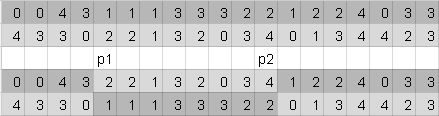
\includegraphics{Imagens/TwoPointsCrossover.png}
		\caption{Exemplo de aplica��o do operador 2x. \\Fonte Autoria Pr�pria}
		\label{fig:twopointscrossover}
	\end{figure}
	
			

	
	\item \textit{Multi Points Crossover} (MPX): Semelhante ao 2X por�m com c pontos, baseado na fun��o $c = int(n * 0.1)$, $n$ � o tamanho da sequ�ncia. O operador MPX � utilizado para promover diversidade estrutural realizando uma mescla rand�mica entre os pais, embora n�o t�o radical quanto o \textit{Uniform  Crossover} \cite{sabar2014automatic}. Um exemplo de aplica��o do operador MPX � apresentado na imagem \ref{fig:multipointscrossover}
	
	
		\begin{figure}[!htb]
			\centering
			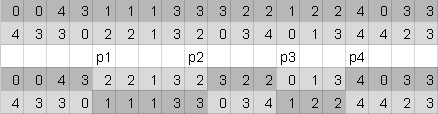
\includegraphics{Imagens/MultiPointsCrossover.png}
			\caption{Exemplo de aplica��o do operador MPX. \\Fonte Autoria Pr�pria}
			\label{fig:multipointscrossover}
		\end{figure}
	\item \textit{Segment Mutation} (SMUT): Altera um n�mero aleat�rio (5 a 7) de genes consecutivos para dire��es distintas. Esta heur�stica introduz grandes mudan�as na conforma��o, e tem uma grande probabilidade de criar colis�es. Um mecanismo de repara��o simples � aplicado no descendente gerado. A imagem \ref{fig:segmentMutation} apresenta um exemplo da aplica��o do SMUT.
	
	\begin{figure}[!htb]
		\centering
		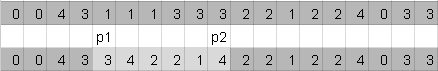
\includegraphics{Imagens/segmentMutation.png}
		\caption{Exemplo de aplica��o do operador SMUT. \\Fonte Autoria Pr�pria}
		\label{fig:segmentMutation}
	\end{figure}
	
	
	\item \textit {Exhaustive Search Mutation} (EMUT): Esta heur�stica seleciona um gene aleat�rio e testa todas as outras dire��es poss�veis e ir� manter a altera��o que conseguir aumentar a qualidade da conforma��o. O \textit{tradeoff} deste operador � demandar 4 avalia��es de \textit{fitness}, as quais devem ser levadas em considera��o. Esta heur�stica tem grande potencial de melhorar o \textit{fitness} de uma conforma��o. 
	
	
	\item \textit{Local Move Operator} (LM): Esta heur�stica troca dire��es entre dois genes aleat�rios consecutivos. Existem algumas condi��es para que esta heur�stica possa ser executada, por exemplo, as novas dire��es n�o podem criar movimentos redundantes. Este operador introduz um "movimento de esquina". A figura \ref{fig:localMoveOperator} apresenta um exemplo da aplica��o do operador LM. 
	
	
	\begin{figure}[!htb]
		\centering
		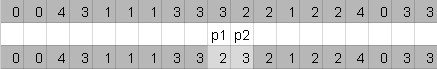
\includegraphics{Imagens/LocalMoveOperator.png}
		\caption{Exemplo de aplica��o do operador LM. \\Fonte Autoria Pr�pria}
		\label{fig:localMoveOperator}
	\end{figure}
	
	
	\item \textit{Loop Move Operator} (LPM): Da mesma maneira que a heur�stica LM, esta heur�stica troca dire��es entre dois genes que est�o a 5 genes de dist�ncia na sequ�ncia, criando um movimento de \textit{loop}. A figura  \ref{fig:loopMoveOperator} apresenta um exemplo da aplica��o do operador LPM.

	
	\begin{figure}[!htb]
		\centering
		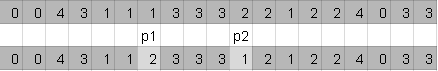
\includegraphics{Imagens/LoopMoveOperator.png}
		\caption{Exemplo de aplica��o do operador LPM. \\Fonte Autoria Pr�pria}
		\label{fig:loopMoveOperator}
	\end{figure}
	
	\item \textit{Opposite Mutation} (OM): Esta heur�stica troca as dire��es, para dire��o oposta, de uma sequ�ncia de genes entre dois genes $(i,j)$ selecionados de maneira aleat�ria. A dire��o 0 ($F$) n�o possui oposta, portanto � mantida. Para exemplificar, suponha esta solu��o hipot�tica para uma sequ�ncia de 5 amino�cidos: $\{0,1,2,1,2\}$. Ela se tornaria $\{0,2,1,2,1\}$. A figura \ref{fig:oppositeMutation} apresenta um exemplo da aplica��o do operador OM.
	
	
	\begin{figure}[!htb]
		\centering
		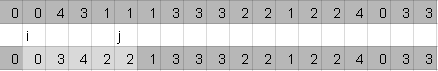
\includegraphics{Imagens/OppositeMutation.png}
		\caption{Exemplo de aplica��o do operador OM. \\Fonte Autoria Pr�pria}
		\label{fig:oppositeMutation}
	\end{figure}
	

	
 \end{itemize} 
 
 
 
 \section{Processo geral da EG proposta} 
 
 As principais etapas da EG proposta ser�o apresentadas nesta se��o.
 Inicialmente uma popula��o de indiv�duos (heur�sticas de alto n�vel: mecanismos de sele��o e crit�rios de aceita��o) � gerada de maneira aleat�ria. O \textit{fitness} da popula��o � calculado inserindo os indiv�duos em um \textit{framework} hiper-heur�stico e o executando por um certo n�mero de itera��es. E de maneira iterativa selecionar indiv�duos pais e aplicar os operadores de cruzamento, \textit{prune}, muta��o, e \textit{duplicate} para gerar descendentes. Para avaliar os descendentes, os seguintes passos s�o executados:
 
 \begin{enumerate}
 	\item Cada indiv�duo � decodificado em um mecanismo de sele��o e um crit�rio de aceita��o (heur�stica de alto n�vel). Os valores, descritos 	para o conjunto terminal na se��o \ref{sec:highlevelheuristics}, de cada heur�stica de baixo n�vel ser�o utilizados como entrada para o mecanismo de sele��o.
 	\item Execu��o do mecanismo de sele��o com objetivo de ordenar o conjunto de heur�sticas de baixo n�vel. As heur�sticas de baixo n�vel s�o ordenadas da maior para a menor baseando-se no resultado da express�o referente ao mecanismo de sele��o. 
 	\item Selecionar de maneira aleat�ria uma solu��o do mecanismo de mem�ria, o qual ser� detalhado na \autoref{sub:MecanismoDeMemoria}. Aplicar a heur�stica de baixo n�vel classificada com o maior valor e calcular a qualidade da solu��o gerada.
 	\item Se a solu��o gerada for melhor do que a atual, a atual � substitu�da. Caso contr�rio a express�o referente ao crit�rio de aceita��o � executada. A solu��o gerada pela heur�stica de baixo n�vel � aceita caso o exponencial natural do valor, retornado pelo crit�rio de aceita��o, seja menor ou igual a 0.5 (a fun��o $e^x$ retorna valores entre 0 e 1). Sabar et al. \cite{sabar2014automatic} menciona que este valor de 0.5 � sugerido pela literatura. 
 	\item Aplicar a heur�stica de baixo n�vel, que foi selecionada pelo mecanismo de sele��o, repetidamente at� que n�o ocorram mais melhorias.
 	\item Se n�o houverem mais melhorias, troca-se a heur�stica de baixo n�vel atual pela segunda melhor classificada, baseando-se no valor retornado pelo mecanismo de sele��o.
 	\item Se o \textit{framework} chegar ao fim da lista de heur�sticas de baixo n�vel, � executado o mecanismo de sele��o novamente e a lista de heur�sticas de baixo n�vel � reordenada. A busca reinicia agora utilizando a heur�stica de baixo n�vel com maior valor para a express�o referente ao mecanismo de sele��o.
 	\item O \textit{framework} proposto continuar� utilizando os componentes da heur�stica de alto n�vel (mecanismo de sele��o e crit�rio de aceita��o) por um tempo pr�-determinado de itera��es.
 	\item A solu��o gerada ao final da busca do \textit{framework} hiper-heur�stico  ser� avaliada para entrar ou n�o no mecanismo de mem�ria.
 \end{enumerate}
 
 O processo da EG ir� parar apenas quando o crit�rio de parada discutido na \autoref{sub:criterioParada} for atingido e ser� retornado o indiv�duo (heur�stica de alto n�vel) que possuir o maior valor de \textit{fitness}. Tamb�m ser� retornada a solu��o ao PDP que tiver maior qualidade no mecanismo de mem�ria.
  
 
 \subsection{Mecanismo de Mem�ria}
 \label{sub:MecanismoDeMemoria}
 
 A maioria dos \textit{frameworks} hiper-heur�sticos propostos na literatura operam sobre uma �nica solu��o \cite{chakhlevitch2008hyperheuristics, burke2013hyper}. Blum et al. \cite{blum2011hybrid} menciona que utilizar uma �nica solu��o pode restringir a capacidade de explorar um espa�o de busca grande e restrito. Dessa maneira, Sabar et al. \cite{sabar2014automatic} prop�s uma abordagem que utiliza um mecanismo de mem�ria, assim como Talbi el al. \cite{talbi2006cosearch}, o qual cont�m um conjunto de solu��es com alta qualidade e diversificadas, atualizado conforme o progresso da busca. Nesta proposta o mecanismo de mem�ria tem a responsabilidade de armazenar solu��es para o problema PDP utilizando a representa��o de coordenadas relativas para o modelo HP-2D. 
 
 \subsubsection{Inicializa��o do Mecanismo de Mem�ria}
 
  Tradicionalmente algoritmos evolutivos inicializam suas popula��es iniciais de maneira aleat�ria, por conta disto  muitas solu��es inv�lidas ao problema PDP, podem ser geradas na inicializa��o. Isto geralmente  ocasiona perda de tempo de processamento, por conta da grande quantidade de conforma��es inv�lidas antes que bons resultados sejam obtidos. Diante disto,  Ben�tez et al. \cite{benitez2015algoritmo} prop�s uma estrat�gia especializada de inicializa��o. Ben�tez et al. \cite{benitez2015algoritmo} inicializou a popula��o de seu algoritmo gen�tico, dividido-a em duas partes. Uma gerada aleatoriamente, com indiv�duos que potencialmente possuem colis�es. E uma segunda parte onde todos os indiv�duos s�o livres de colis�es. Uma configura��o � utilizada para definir a propor��o entre as duas partes da popula��o inicial. Para garantir que os indiv�duos n�o possuam colis�es, uma estrat�gia de \textit{backtracking} deve ser utilizada. Nesta proposta, pretende-se utilizar uma estrat�gia similar, adaptada ao modelo HP-2D.  A estrat�gia de inicializa��o com \textit{backtracking} ir� come�ar posicionando o primeiro amino�cido na posi��o 0,0. Para posicionar o pr�ximo amino�cido, um movimento � selecionado de maneira aleat�ria. Caso o movimento cause uma colis�o, este movimento ser� marcado como uma m� escolha e um novo movimento � selecionado aleatoriamente (do conjunto que restou sem os movimentos marcados como m�s escolhas). Caso todos os movimentos estejam marcados como m� escolha, a estrat�gia de \textit{backtracking} ir� retornar de maneira recursiva para o amino�cido anterior e marcar a escolha em quest�o como uma m� escolha. A estrat�gia de \textit{backtracking} termina quando gerar uma conforma��o que n�o possua colis�es.
 
   %As poss�veis conforma��es podem ser representadas por um caminho em um grafo orientado estruturado como uma �rvore. Consequentemente, cada n� da �rvore representa uma solu��o candidata parcial $c$, desde o primeiro amino�cido at� o �ltimo sendo considerado. Portanto, um caminho at� um n� folha representa uma conforma��o completa. As arestas do grafo representam o movimento de cada amino�cido relativo a seu predecessor.
  

 
 \subsubsection{Atualiza��o do Mecanismo de Mem�ria}
 Para cada indiv�duo (heur�stica de alto n�vel) ser� selecionada de maneira aleat�ria uma solu��o do mecanismo de mem�ria e a busca ir� iniciar em torno desta solu��o, quando o \text{framework} hiper-heur�stico atingir o seu n�mero m�ximo de itera��es a solu��o final tem que ser avaliada para verificar sua qualidade e diversidade. A qualidade de uma solu��o para o PDP utilizando o modelo HP � inversamente proporcional � quantidade de intera��es entre amino�cidos hidrof�bicos. Portanto a qualidade de uma solu��o � dada pela quantidade de itera��es H-H multiplicada por -1, conforme descrito na subse��o \ref{subsubsection:modeloHP}.  As solu��es geradas que tiverem a qualidade maior que todas as solu��es contidas no mecanismo de mem�ria substituir�o a solu��o que tiver menor similaridade segundo a dist�ncia de \textit{Hamming} \cite{hamming1950error}. Se a qualidade de uma solu��o gerada n�o for maior que todas as solu��es, mas melhor em rela��o a um sub-conjunto do mecanismo de mem�ria, esta substituir� a solu��o que tiver menor qualidade e menor similaridade do sub-conjunto. E por fim se a qualidade da solu��o gerada for pior que todas contidas no mecanismo de mem�ria, esta � descartada. A similaridade � considerada a fim de manter a diversidade entre as solu��es.  
 
 
 
 
% Esta representa��o possibilita a gera��o de solu��es inv�lidas, que possuem colis�es. Tradicionalmente algoritmos evolutivos inicializam suas popula��es iniciais de maneira aleat�ria, por conta disto  muitas solu��es inv�lidas ao problema PDP, podem ser geradas na inicializa��o. Isto geralmente  ocasiona perda de tempo de processamento, por conta da grande quantidade de conforma��es inv�lidas antes que bons resultados sejam obtidos. Diante disto,  Ben�tez et al. \cite{benitez2015algoritmo} prop�s uma estrat�gia especializada de inicializa��o. Ben�tez et al. \cite{benitez2015algoritmo} inicializou a popula��o de seu algoritmo gen�tico, dividido-a em duas partes. Uma gerada aleatoriamente, com indiv�duos que potencialmente possuem colis�es. E uma segunda parte onde todos os indiv�duos s�o livres de colis�es. Uma configura��o � utilizada para definir a propor��o entre as duas partes da popula��o inicial. Para garantir que os indiv�duos n�o possuam colis�es, uma estrat�gia de \textit{backtracking} deve ser utilizada. Nesta proposta, pretende-se utilizar uma estrat�gia similar, adaptada ao modelo HP-2D. As poss�veis conforma��es podem ser representadas por um caminho em um grafo orientado estruturado como uma �rvore. Consequentemente, cada n� da �rvore representa uma solu��o candidata parcial $c$, desde o primeiro amino�cido at� o �ltimo sendo considerado. Portanto, um caminho at� um n� folha representa uma conforma��o completa. As arestas do grafo representam o movimento de cada amino�cido relativo a seu predecessor.
 
 % A figura \ref{fig:backtrackInit}  apresenta um fragmento do espa�o de busca para uma cadeia hipot�tica com 5 amino�cidos. O espa�o de busca completo � grande totalizando  $5^4=625$ possibilidades, e n�o pode ser apresentado por quest�es de visualiza��o.
 
 % 	\begin{figure}[!htb]
 % 		\centering
 % 		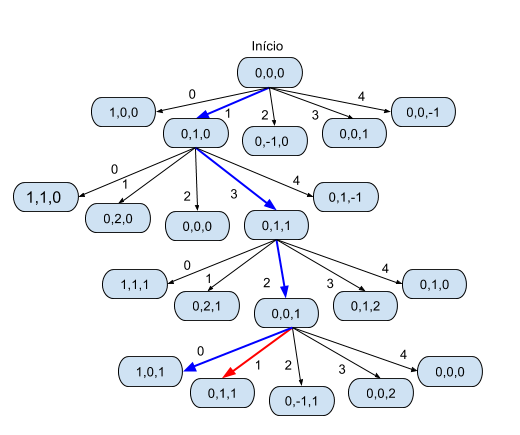
\includegraphics[scale=0.8]{Imagens/BacktrackingInit.png}
 % 		\caption{Fragmento do espa�o de busca para o modelo HP. \\Fonte Autoria Pr�pria}
 % 		\label{fig:backtrackInit}
 % 	\end{figure}
 
 % 	Na figura \ref{fig:backtrackInit} (TODO: arrumar imagem e explica��o para o HP-2D) o caminho apresentado pelas setas azuis representa uma solu��o que gera uma conforma��o v�lida (sem colis�es). A seta vermelha demonstra que se caso o ultimo passo fosse alterado de 0 para 1. Esta altera��o causaria uma conforma��o inv�lida, pois posicionaria o ultimo amino�cido na posi��o 0,1,1 a qual j� havia sido ocupada no segundo passo. 
% A estrat�gia de inicializa��o com \textit{backtracking} ir� come�ar posicionando o primeiro amino�cido na posi��o 0,0. Para posicionar o pr�ximo amino�cido, um movimento � selecionado de maneira aleat�ria. Caso o movimento cause uma colis�o, este movimento ser� marcado como uma m� escolha e um novo movimento � selecionado aleatoriamente (do conjunto que restou sem os movimentos marcados como m�s escolhas). Caso todos os movimentos estejam marcados como m� escolha, a estrat�gia de \textit{backtracking} ir� retornar de maneira recursiva para o amino�cido anterior e marcar a escolha em quest�o como uma m� escolha. A estrat�gia de \textit{backtracking} termina quando gerar uma conforma��o que n�o possua colis�es.
 
 
 % 	e selecionando de maneira aleat�ria o movimento para o pr�ximo 
 % 	
 % 	
 % 	amino�cido. Caso este movimento cause uma colis�o (seja posicionado em uma regi�o da grade que j� havia um amino�cido) o \textit{backtracking} entra em cena percorrendo a �rvore de maneira recursiva 
 
 
 
 % Para cada solu��o, uma matriz de frequ�ncia � associada afim de medir a diversidade da solu��o. A matriz de frequ�ncia ir� armazenar a frequ�ncia que cada amino�cido foi atribu�do para cada uma das dire��es poss�veis $\{0,1,2,3,4\}$. A figura \ref{fig:frequencyMatrix} apresenta um exemplo de uma matriz de frequ�ncia para uma cadeia hipot�tica $HPPHHHP$ de 7 amino�cidos. Observando a figura  \ref{fig:frequencyMatrix} � poss�vel notar que o amino�cido 0 foi atribu�do a dire��o E (3), que significa esquerda, duas vezes, tr�s vezes para a dire��o D (4), que significa direita e nenhuma vez para as dire��es F(0), D(1) e B(2). 
 
 
 % 	\begin{figure}[!htb]
 % 		\centering
 % 		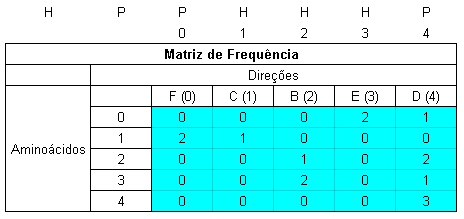
\includegraphics[scale=0.8]{Imagens/FrequencyMatrix.png}
 % 		\caption{Fragmento BLAH. \\Fonte Autoria Pr�pria}
 % 		\label{fig:frequencyMatrix}
 % 	\end{figure}
 %
 
 %Para avaliar a diversidade ser� utilizada a entropia da informa��o.  As equa��es \ref{equation:entropy1} e \ref{equation:entropy2} exemplificam o c�lculo de entropia.
 
% \begin{equation}
%	 \label{equation:entropy1}
% 	 \epsilon_i = \frac{\sum\limits_{i=1}^e \frac{e_{ij}}{m}  . \log \frac{e_{ij}}{m}}{-log~e}
% \end{equation}
% 
%  \begin{equation}
%  	 \label{equation:entropy2}
%  \epsilon = \frac{\sum\limits_{i=1}^e \epsilon_i}{e}
%  \end{equation}
%  
%	 \noindent$e_{ij}$ � a frequ�ncia de aloca��o do amino�cido $i$ para a dire��o $j$; \\
%	 $m$ � o n�mero de objetos; \\
%	 $\epsilon_i$ representa a entropia para o amino�cido $i$;
%	 $\epsilon$ representa a entropia para uma solu��o completa (todos os amino�cidos) ($0 <= \epsilon_i <= 1$). 
% 

 



\section{Considera��es Finais}
\label{Metodologia:ConsideracoesFinais}

Neste cap�tulo foram discutidos os principais aspectos relativos a metodologia para aplicar a evolu��o gramatical com objetivo de gerar heur�sticas de alto n�vel de um \text{framework} hiper-heur�stico para o PDP. Inicialmente foi discutido que esquema de codifica��o utilizado para representar as solu��es ao PDP ser�o coordenadas relativas. Em seguida, foi apresentada a gram�tica desenvolvida para gerar as heur�sticas de alto n�vel. Os componentes terminais da gram�tica representam diferentes aspectos estat�sticos referente ao hist�rico das aplica��es das heur�sticas de baixo n�vel. Fun��es matem�ticas simples tamb�m comp�em a gram�tica e combinadas com os aspectos estat�sticos gerar�o diferentes heur�sticas de alto n�vel. Posteriormente, a fun��o de \textit{fitness} para avaliar as heur�sticas de alto n�vel e o crit�rio de parada foram da EG foram introduzidos. As heur�sticas de baixo n�vel tamb�m foram apresentadas. E finalmente o processo geral desta proposta foi apresentado incluindo os aspectos referente ao mecanismo de mem�ria. 
O pr�ximo cap�tulo apresenta as atividades j� realizadas e as atividades a serem realizadas assim como, um cronograma para realiza��o das atividades restantes.


%\input{Resultados}
\chapter{Proposta de Trabalho}
\label{Proposta de Trabalho}

Este cap�tulo tem por objetivo apresentar as atividades necess�rias para este trabalho, bem como o cronograma que ser� seguido. As atividades j� realizadas s�o apresentadas na Se��o \ref{Proposta de Trabalho:Atividades Realizadas}, as atividades que ser�o realizadas s�o apresentadas na Se��o~\ref{Proposta de Trabalho:Atividades a Serem Realizadas} e o cronograma proposto para as atividades � apresentado na Se��o~\ref{Proposta de Trabalho:Cronograma de Trabalho}.

\section{Atividades Realizadas}
\label{Proposta de Trabalho:Atividades Realizadas}

A seguir s�o apresentadas as atividades que j� foram realizadas durante o per�odo de mestrado:

\begin{enumerate}
	\item \textbf{Pesquisa de Trabalhos Relacionados} -- Foi realizada uma pesquisa de trabalhos relacionados, a qual foi apresentada no Cap�tulo \ref{Trabalhos Relacionados};
	\item \textbf{Busca por Estilos Arquiteturais a serem utilizados} -- Foi conduzida uma busca com o objetivo de encontrar alguns estilos arquiteturais para serem utilizados juntamente com LPS neste trabalho. A rela��o de alguns estilos arquiteturais encontrados com base em afirma��es de autores foi apresentada no Cap�tulo~\ref{Trabalhos Relacionados};
	\item \textbf{An�lise de Operadores} -- Foi conduzida uma an�lise dos operadores apresentados na Se��o~\ref{Search-based Software Design:Operadores} com o objetivo de verificar quais deles poderiam corromper um estilo arquitetural.
	\item \textbf{Proposta de Operadores com Restri��es} -- Baseando-se na an�lise realizada na Atividade 3, foram propostos operadores com restri��es associados aos estilos arquiteturais. Os operadores com restri��es foram criados para os estilos arquiteturais selecionados na Atividade 2. Os operadores com restri��es propostos foram apresentados no Cap�tulo~\ref{Operadores de Mutacao e Estilos Arquiteturais} e ser�o implementados no m�dulo OPLA-Arch-Styles.
\end{enumerate}

At� o momento, apenas pseudoc�digos para os operadores com restri��es foram desenvolvidos, por�m implementa��es concretas ser�o realizadas com o objetivo de valid�-los. Com base nisso, algumas atividades a serem realizadas foram identificadas e s�o apresentadas na pr�xima se��o.

\section{Atividades a Serem Realizadas}
\label{Proposta de Trabalho:Atividades a Serem Realizadas}

As atividades a serem realizadas s�o apresentadas a seguir:

\begin{enumerate}
	\item \textbf{Implementa��o do m�dulo OPLA-Arch-Styles} -- O m�dulo OPLA-Arch-Styles apresentado na Se��o \ref{Search-based Software Design:OPLA-Tool} dever� ser implementado do modo que foi apresentado na Figura~\ref{AspectosImplementacao:Figura:OPLA-Arch-Styles}. Os operadores com restri��es de estilos arquiteturais propostos na Se��o~\ref{Operadores de Mutacao e Estilos Arquiteturais} dever�o ser implementados, de modo que a aplica��o dos mesmos seja totalmente autom�tica;
	\item \textbf{Incorpora��o do m�dulo OPLA-Arch-Styles na ferramenta OPLA-Tool} -- O m�dulo OPLA-Arch-Styles dever� ser incorporado � ferramenta OPLA-Tool, realizando a integra��o com os demais m�dulos da ferramenta conforme ilustrado na Figura~\ref{Search-based Software Design:Figura:Modulos da OPLA-Tool};
	\item \textbf{Valida��es Experimentais} -- O m�dulo OPLA-Arch-Styles dever� ser validado experimentalmente utilizando LPSs reais que sigam os estilos arquiteturais escolhidos. Um exemplo de LPS real que segue o estilo arquitetural em camadas � a AGM~\cite{seiAGM}, que foi apresentada no Cap�tulo~\ref{Operadores de Mutacao e Estilos Arquiteturais};
	\item \textbf{Elabora��o de Artigos Cient�ficos} -- Ap�s a Atividade 3, poder� ser realizada a reda��o de artigos cient�ficos com o objetivo de publicar os resultados alcan�ados;
	\item \textbf{Reda��o da Disserta��o};
	\item \textbf{Defesa da Disserta��o}.
\end{enumerate}


\section{Cronograma de Trabalho}
\label{Proposta de Trabalho:Cronograma de Trabalho}

O tempo previsto para a realiza��o das atividades apresentadas na Se��o \ref{Proposta de Trabalho:Atividades a Serem Realizadas} � de 12 meses e o planejamento para esse per�odo � apresentado na Tabela \ref{Proposta de Trabalho:Tabela:Cronorgrama de Atividades a Serem Realizadas}.

\begin{table}[!htb]
	\renewcommand{\arraystretch}{1.2}
	\centering
	\caption{Cronograma de Atividades a Serem Realizadas}
	\label{Proposta de Trabalho:Tabela:Cronorgrama de Atividades a Serem Realizadas}
	\begin{tabular}{c|c|c|c|c|c|c|c|c|c|c|c|c}
		\toprule
		\multirow{4}{*}{\textbf{Atividade}} & \multicolumn{10}{c}{\textbf{Ano}} \\ 
		\cline{2-13} 
		& \multicolumn{10}{c|}{\textbf{2014}} & \multicolumn{2}{c}{\textbf{2015}} \\ 
		\cline{2-13} 
		& \multicolumn{10}{c}{\textbf{M�s}} \\ 
		\cline{2-13} 
		& \textbf{03} & \textbf{04} & \textbf{05} & \textbf{06} & \textbf{07} & \textbf{08} & \textbf{09} & \textbf{10} & \textbf{11} & \textbf{12} & \textbf{01} & \textbf{02}\\ 
		\bottomrule
		\textbf{1} & \cellcolor{darkgray} & \cellcolor{darkgray} & \cellcolor{darkgray} & \cellcolor{darkgray} & \cellcolor{darkgray} & & & & & & & \\ \hline
		\textbf{2} & & & & \cellcolor{darkgray} & \cellcolor{darkgray} & \cellcolor{darkgray} & & & & & & \\ \hline
		\textbf{3} & & & & & & \cellcolor{darkgray} & \cellcolor{darkgray} & \cellcolor{darkgray} & \cellcolor{darkgray} & & & \\ \hline
		\textbf{4} & & & & & & & & \cellcolor{darkgray} & \cellcolor{darkgray} & \cellcolor{darkgray} & \cellcolor{darkgray} & \cellcolor{darkgray} \\ \hline
		\textbf{5} & & & & & & & & \cellcolor{darkgray} & \cellcolor{darkgray} & \cellcolor{darkgray} & \cellcolor{darkgray} & \cellcolor{darkgray} \\ \hline
		\textbf{6} & & & & & & & & & & & & \cellcolor{darkgray} \\
		\toprule
	\end{tabular}
\end{table}

\newpage
% Bibliografia
\addcontentsline{toc}{chapter}{\MakeUppercase{Refer�ncias}}
\bibliographystyle{brazil}
\bibliography{bibliografia}

\appendix

\singlespacing
\makecapadissertacao

\end{document}